% !TEX root = dissertation_BB.tex
%% spellcheck-language en-US

%  ####
%      #
%   ###
%  #
%  #####

\chapter{Dual Mouse-SPIM}

\graphicspath{{./figures/2_DualMouse/}}

\label{ch:DualMouse}
% \section{Challenges in imaging mouse pre-implantation development}
  % mammalian development
  % chromosome segregation
  % cell specification
  % symmetry breaking
  % signaling pathways
  % human infertility
  % congenital diseases 

  % advantages:
  %   immersion liquid and culture medium separated
  %   open-top sample holder allow standard microdrop \textit{in vitro} embryo culture
  %   row of embryos - high throughput
  %   dual color imaging
  %   environmental chamber allows live imaging for 3 days, every 

  % follow chromosomes by tracking kinetochores

  % from lattice paper: ``because photodamage mechanisms that scale supralinearly with peak intensity have been identified for both visible \cite{donnert_major_2007} and two-photon \cite{ji_high-speed_2008} excitation."

  % move this to chapter DualMouse -->
Unraveling the secrets of mammalian development has been a long standing challenge for developmental biologists and medical professionals alike. 
This phase of early life is an incredibly complex and dynamic process spanning through large scales in space and time. Subcellular processes at the nanoscale are happening in the range of milliseconds or shorter, while whole embryo reorganizations and tissue migration events take place over the course of hours \cite{gilbert_developmental_2013}. Resolving these processes presents a true challenge, since to understand the underlying mechanisms, molecular specificity is just as crucial as high spatial and temporal resolution.
% <--
As we have seen in \autoref{ch:intro}, live imaging of mouse embryonic development is an especially challenging task, but light-sheet microscopy can offer a good solution owing to its gentle optical sectioning and fast image acquisition. The Mouse-SPIM \cite{strnad_inverted_2016} introduced earlier (\autoref{ch:mouse-intro}) also solves the issue of live imaging with its inverted design: the embryos are held by a foil which not only allows easy sample handling but also acts as a barrier that isolates the embryos from the immersion medium.

As all microscopes, the Mouse-SPIM also had to make a compromise: although its design allows for long-term live imaging, it only has a single detection view, as rotation is not possible with the sample mounting trays. Due to this configuration, its resolution is inherently anisotropic, having an axial-to-lateral resolution ratio of around 3. Although this is sufficient for many applications, such as cell tracking, for detecting subcellular features it might be limiting. One such example is chromosome tracking, which could shed light on chromosome missegregation mechanisms in the early embryonic development, which is the cause of many congenital diseases also affecting humans.

In this chapter, we present a novel light-sheet microscope developed to address the above challenges by using two high NA objectives for subcellular isotropic resolution and low-light imaging, while offering multi-view detection without the need to rotate the samples. The microscope is designed to be live imaging compatible, offering new perspectives in the research of mouse embryonic development. This chapter will describe the design concepts for the microscope, the optical layout, alignment strategies, the results of various performance measurements, and its multi-view imaging capabilities. 

  %#######  ########  ######  ####  ######   ##    ## 
  %#     ## ##       ##    ##  ##  ##    ##  ###   ## 
  %#     ## ##       ##        ##  ##        ####  ## 
  %#     ## ######    ######   ##  ##   #### ## ## ## 
  %#     ## ##             ##  ##  ##    ##  ##  #### 
  %#     ## ##       ##    ##  ##  ##    ##  ##   ### 
  %#######  ########  ######  ####  ######   ##    ## 

\section{Microscope design concept}
\label{sec:120concept}

  \begin{figure}
    \centering
    \begin{subfigure}{0.49\textwidth}
      \centering
      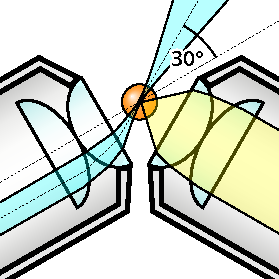
\includegraphics[page=1,width=0.8\textwidth]{objectiveCloseup}
    \end{subfigure}
    \begin{subfigure}{0.49\textwidth}
      \centering
      \includegraphics[page=2,width=0.8\textwidth]{objectiveCloseup}
    \end{subfigure}
    \bcaption[Dual view concept with high NA objectives]{To achieve multi-view detection while maximizing resolution and light collection efficiency, two high NA objectives are placed in a \SI{120}{\degree} arrangement. The sample (orange) is held from below by a thin FEP foil. To be able to overlap the light-sheet with the focal plane, the light-sheet is tilted by \SI{30}{\degree}. The objectives are used in an alternating sequence for illumination and detection.}
    \label{fig:objectiveCloseup}
  \end{figure}

  As the limiting factor for subcellular imaging with the original Mouse-SPIM is the poor axial resolution relative to the lateral, our first aim was to increase the axial resolution to ideally reach the lateral resolution. A common way to reach isotropic resolution is to image a specimen from multiple directions, and combine the resulting images by multi-view deconvolution \cite{swoger_multi-view_2007,temerinac-ott_multiview_2012, preibisch_efficient_2014}. This has the benefit that the high-resolution information from one view can complement the low axial resolution of the other view, thus providing better resolution in all three directions.

  As described in \autoref{ch:intro}, many SPIM implementations allow for recording multiple views either by rotating the sample, or by surrounding the sample with multiple objectives that are used for detection (\autoref{fig:spim_zoo}). For our setup, following the sample mounting technique of the original Mouse-SPIM, we wanted to keep the open-top sample mounting possibility, as this was proven to be highly compatible with mouse embryo imaging. To achieve multi-view detection in this configuration, we designed a setup where both objectives can be used for illumination and detection in a sequential manner, inspired by previous symmetrical SPIM designs \cite{balazs_development_2013, wu_spatially_2013}.

  To achieve the highest possible resolution from two views, the core of our design is based on the symmetric arrangement of two Nikon CFI75 Apo LWD 25x water-dipping objectives, with a numerical aperture of 1.1. Due to the large light collection angle of these objectives, we arrange them in \SI{120}{\degree} instead of the conventional \SI{90}{\degree} used for light-sheet imaging. As the light-sheet still needs to coincide with the imaging focal plane of the objectives, we tilt the light-sheet by \SI{30}{\degree} (\autoref{fig:objectiveCloseup}). Due to the low NA of the light-sheet, this is possible without affecting illumination quality.

  This \SI{120}{\degree} arrangement has several benefits when compared to the traditional \SI{90}{\degree} configuration. When placing the objectives in \SI{90}{\degree} the largest possible light collection half-angle for an objective can be $\alpha_{max,90} =\SI{45}{\degree}$, and the corresponding NA is $\na_{max,90} = n \cdot \sin \alpha_{max,90} = 0.94$, where $n=1.33$ is the refractive index of water. Considering that this is an idealized case, the practically available highest NA is only 0.8. For a \SI{120}{\degree} arrangement, the theoretical maximum is $\na_{max,120} = n \cdot \sin (\SI{120}{\degree} /2) = 1.15$, with a practical maximum NA of 1.1.

  Although the resolution won't be completely isotropic when combining the images from two \SI{120}{\degree} views (\autoref{fig:psf-rot}), as it is for \SI{90}{\degree} views, due to the higher maximum NA possible, the resolution can be higher in the \SI{120}{\degree} case. When simulating the combined multi-view PSFs (\autoref{fig:psf-rot}), for 0.8 NA objectives in \SI{90}{\degree} the axial and lateral resolutions are both \SI{317}{nm}; while for two 1.1 NA objectives in \SI{120}{\degree} the axial resolution will be identical, \SI{317}{nm}, and the lateral will be better, \SI{193}{nm}.
  
  Although this difference in resolution may seem marginal, the \SI{120}{\degree} configuration has another advantage in light collection efficiency. Collecting as much of the fluorescence signal as possible is crucial in live imaging applications, due to the limited available photon budget (see \autoref{fig:tradeoffs} and \cite{laissue_assessing_2017}). Collecting more light from the sample allows to image faster with the same contrast, or allows to reduce the illumination power and maintain the imaging speed. As light collection efficiency depends on the solid angle subtended by the detection lens, (see Appendix \autoref{app:lightEff}), a 1.1 NA objective can collect twice as many photons as a 0.8 NA objective, which gives the \SI{120}{\degree} setup a clear edge in low-light imaging.

  \begin{figure}
    \centering
    \begin{subfigure}[t]{0.45\textwidth}
      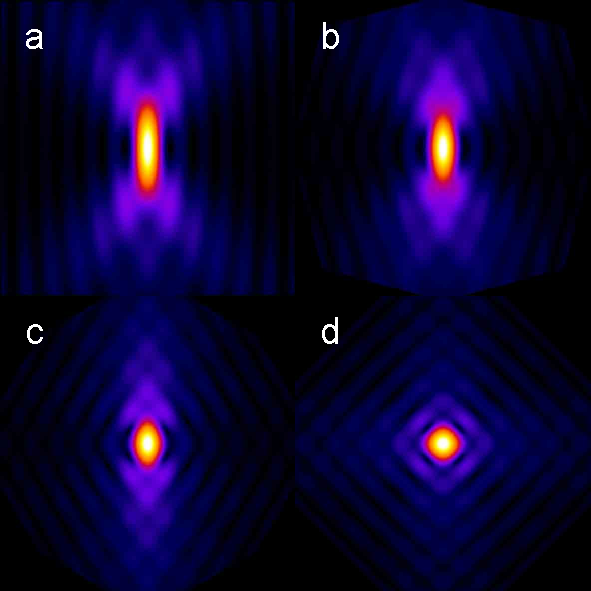
\includegraphics[width=\columnwidth]{simu/psf}
    \end{subfigure}	
    \begin{subfigure}[b]{0.5\textwidth}
    \qquad e
    
      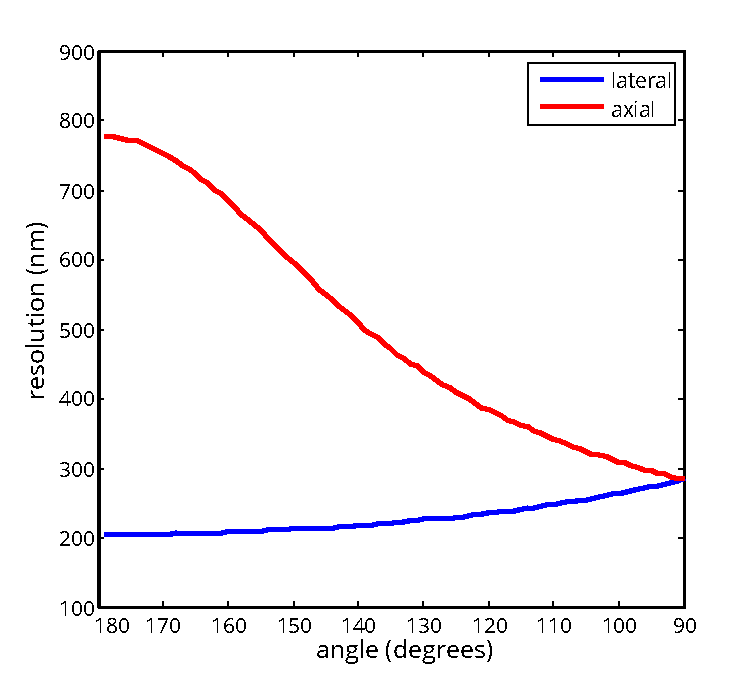
\includegraphics[width=\columnwidth]{simu/resolution}
    \end{subfigure}
    \bcaption[Lateral and axial resolution of a multi-view optical system]{a) Simulated PSF for a single view. b)--d) Simulated compound PSF of two views aligned in b) 150, c) 120 and d) 90 degrees to each other. e) Axial and lateral resolution of a dual-view setup depending on the rotation angle of the two objectives. Parameters used for calculations: NA=1.1, $\lambda_{ex}=488$nm, $\lambda_{det}=510$nm, $n=1.333$ for water immersion.}
    \label{fig:psf-rot}
  \end{figure}


  % Due to the sample mounting constraints (\autoref{fig:preMouse}) when imaging mouse embryos, it is not feasible to surround the sample with objectives, as it can be done with other specimens, such as a \textit{Drosphila} embryo. Rotation is also not possible, since the sample holder is open on the top. To still allow for multi-view imaging, one possibility is to use two identical objectives, both capable of illumination and detection, in a symmetrical configuration \cite{balazs_development_2013,wu_spatially_2013}

  % In order to address the challenges outlined in the previous section, we propose a new light-sheet microscope design for imaging pre-implantation development at high resolution. The design is guided by the following requirements:
  % \begin{enumerate}
  %   \item subcellular, isotropic resolution
  %   \item high light collection efficiency
  %   \item live embryo compatible
  % \end{enumerate}
    

  \subsection{Light-sheet design}
    \label{sec:ls-design}
    To allow for flexibility in the field of view height, to achieve even illumination, reduced stripes, and have the potential for confocal line detection, we opted to use the beam-scanning technique to generate a virtual light-sheet. The effective focal length of the Nikon 25x objective, given the \SI{200}{mm} focal length tube lens is
    \begin{equation}
    f_{o} = \frac{f_{tl}}{M} = \frac{200\text{  mm}}{25} = 8 \text{  mm},
    \end{equation}
    and the back aperture diameter is $d = \SI{17.6}{mm}$.
    
    To generate the tilted light-sheet as shown on \autoref{fig:objectiveCloseup}, the illumination beam will need to be displaced in the back focal plane by
    \begin{equation}
      \delta = f_o \cdot \tan \SI{30}{\degree} = \SI{4.62}{mm}
    \end{equation}
    
    Since the Gaussian beam is not uniform, only a smaller portion of it can be used to maintain an even illumination (\autoref{fig:fov}). Because the size of an early mouse embryo is around \SI{80}{\micro m}, we require the length and the height of the light-sheet to be at least \SI{100}{\micro m}.
    

    \subsubsection{The length and thickness of the light-sheet}
    
      As we saw in \autoref{sec:dimensions}, the length of the light-sheet is determined by the Rayleigh-range of the beam in the $zy$-plane. Since $l_{\mathrm{FOV}}=2\cdot z_{R}=\SI{100}{\micro m}$
      \begin{equation}
        z_{R}=\SI{50}{\micro m}.
      \end{equation}
      Since the Rayleigh range and the diameter of the beam waist are coupled, the light-sheet thickness can be calculated after rearranging \autoref{eq:rayleigh}:
      \begin{equation}
        2\cdot W_{0} = 2\cdot \sqrt{\frac{z_R \cdot \lambda}{\pi}} = \SI{5.57}{\micro m}
      \end{equation}
      when $\lambda=\SI{488}{nm}$ for GFP excitation. As the beam width for these calculations is defined as $1/e^2$ of the peak intensity, we also calculate the more commonly used full width at half maximum (FWHM):
      \begin{equation}
        \mathrm{FWHM} = W_0 \cdot \sqrt{2 \ln 2} = \SI{3.28}{\micro m}.
      \end{equation}      
      From this, the divergence angle of the beam is
      \begin{equation}
        \theta_0 = \frac{\lambda}{\pi W_{0,y}} = \SI{55.74}{mrad} = \SI{3.196}{\degree}
      \end{equation}
      This means, the numerical aperture needed to produce this light-sheet is:
      \begin{equation}
        \NA_{ls} = n\cdot \sin(\theta _0) = 0.0743
      \end{equation}
      Since $\NA=1.1$, the diameter of the back aperture is $d=\SI{17.6}{mm}$ and the divergence angle $\theta_0 \ll 1$, using paraxial approximation, the necessary beam width at the back focal plane in the $y$ direction is
      \begin{equation}
        b_y = d \cdot \frac{\NA_{ls}}{\NA} = \SI{1.19}{mm}
      \end{equation}
      Thus, to generate a light-sheet with appropriate length to cover a whole mouse pre-implantation embryo, the laser beam diameter should be $b=\SI{1.19}{mm}$. Larger diameters will result in a more focused beam and a shorter light-sheet, while a smaller diameter beam will have worse optical sectioning capabilities, but will provide a larger field of view.

    \subsubsection{The height of the light-sheet}
    
    The height of the light-sheet can be adjusted by changing the beam scanning amplitude with the galvanometric mirror (also referred to as scanner). To scan the entire height of the field of view of $h_{\mathrm{FOV}} = \SI{270}{\micro m}$, the scanning angle range at the back focal plane of the objective will need to be $ \theta = \tan^{-1}(h_{\mathrm{FOV}}/2/f_o) = \pm \SI{0.967}{\degree}$.


      

 %######  ########  ######## ####  ######   ######  
%#     ## ##     ##    ##     ##  ##    ## ##    ## 
%#     ## ##     ##    ##     ##  ##       ##       
%#     ## ########     ##     ##  ##        ######  
%#     ## ##           ##     ##  ##             ## 
%#     ## ##           ##     ##  ##    ## ##    ## 
 %######  ##           ##    ####  ######   ######  

\section{Optical layout}
  
  Based on the requirements and other considerations shown in the previous sections, the microscope was designed in three main parts: 1) the core unit (green), 2) illumination branches (blue) and 3) detection branches (yellow, \autoref{fig:fullSchematics}). The aim when integrating these units together was to allow for high level of flexibility with robust operation, while also keeping efficiency in mind. After finalizing the concept, the mechanical layout of the microscope was designed in SolidWorks.


  % \begin{figure}[bth]
  %   \centering
  %   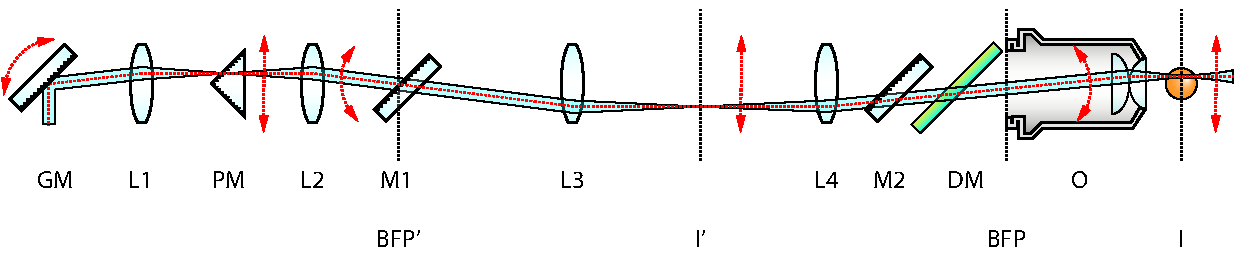
\includegraphics[page=1,width=1\textwidth]{schematicsLinear}
  %   \bcaption[Simplified schematics for illumination]{}
  %   \label{fig:schematicsLinear}
  % \end{figure}
  \begin{figure}
    \centering
    \begin{subfigure}{\textwidth}
      \centering
      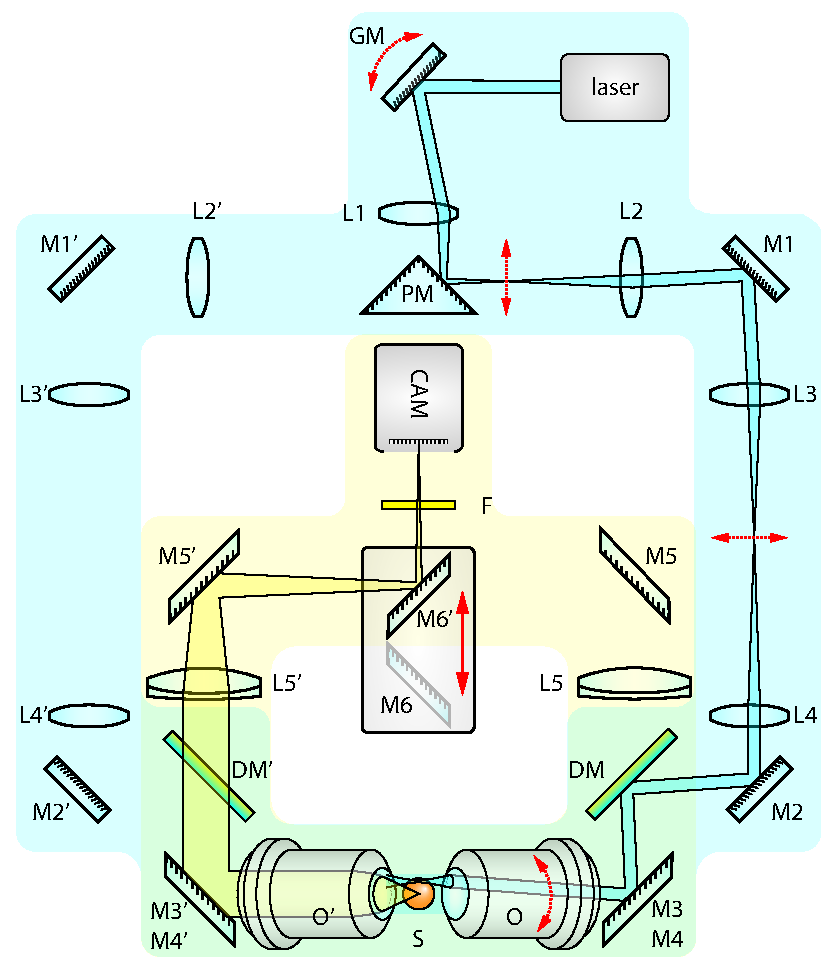
\includegraphics[page=1,width=0.9\textwidth]{fullSchematics}
    \end{subfigure}
    \begin{subfigure}{\textwidth}
      \centering
      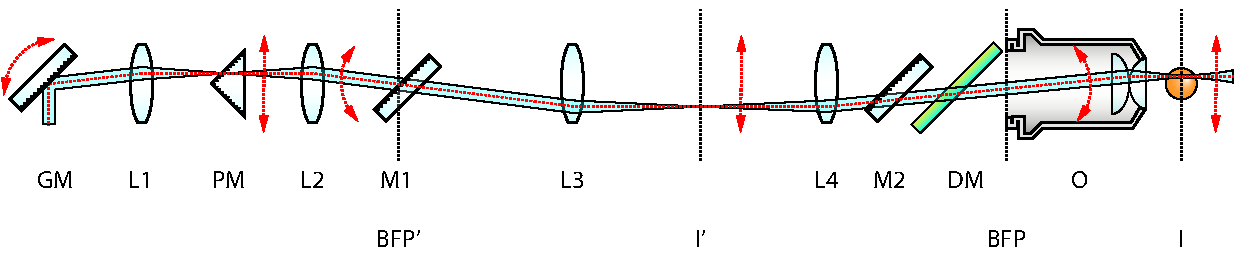
\includegraphics[page=1,width=1\textwidth]{schematicsLinear}
    \end{subfigure}
    
    \bcaption[Dual Mouse-SPIM optical layout]{The microscope consists of two main parts, the illumination branches (blue) and detection branches (yellow). For both illumination and detection there are two identical paths implemented. The illumination direction can be changed by applying a different offset to the galvanometric mirror, which in turn will direct the beam to the opposite face of the prism mirror. L1 and L2 will then image the scanner on M1. Using L3 as a scan lens, and L4 as a tube lens, the scanned beam is coupled into the objective path by a quad band dichroic mirror.
    CAM -- camera, DM -- dichroic mirror, FW -- filter wheel, L -- lens, M -- mirror, O -- objective, PM -- prism mirror, S -- sample}
    \label{fig:fullSchematics}
  \end{figure}


  \subsection{Core unit}
  \label{sec:core}
    \begin{figure}
      \centering
      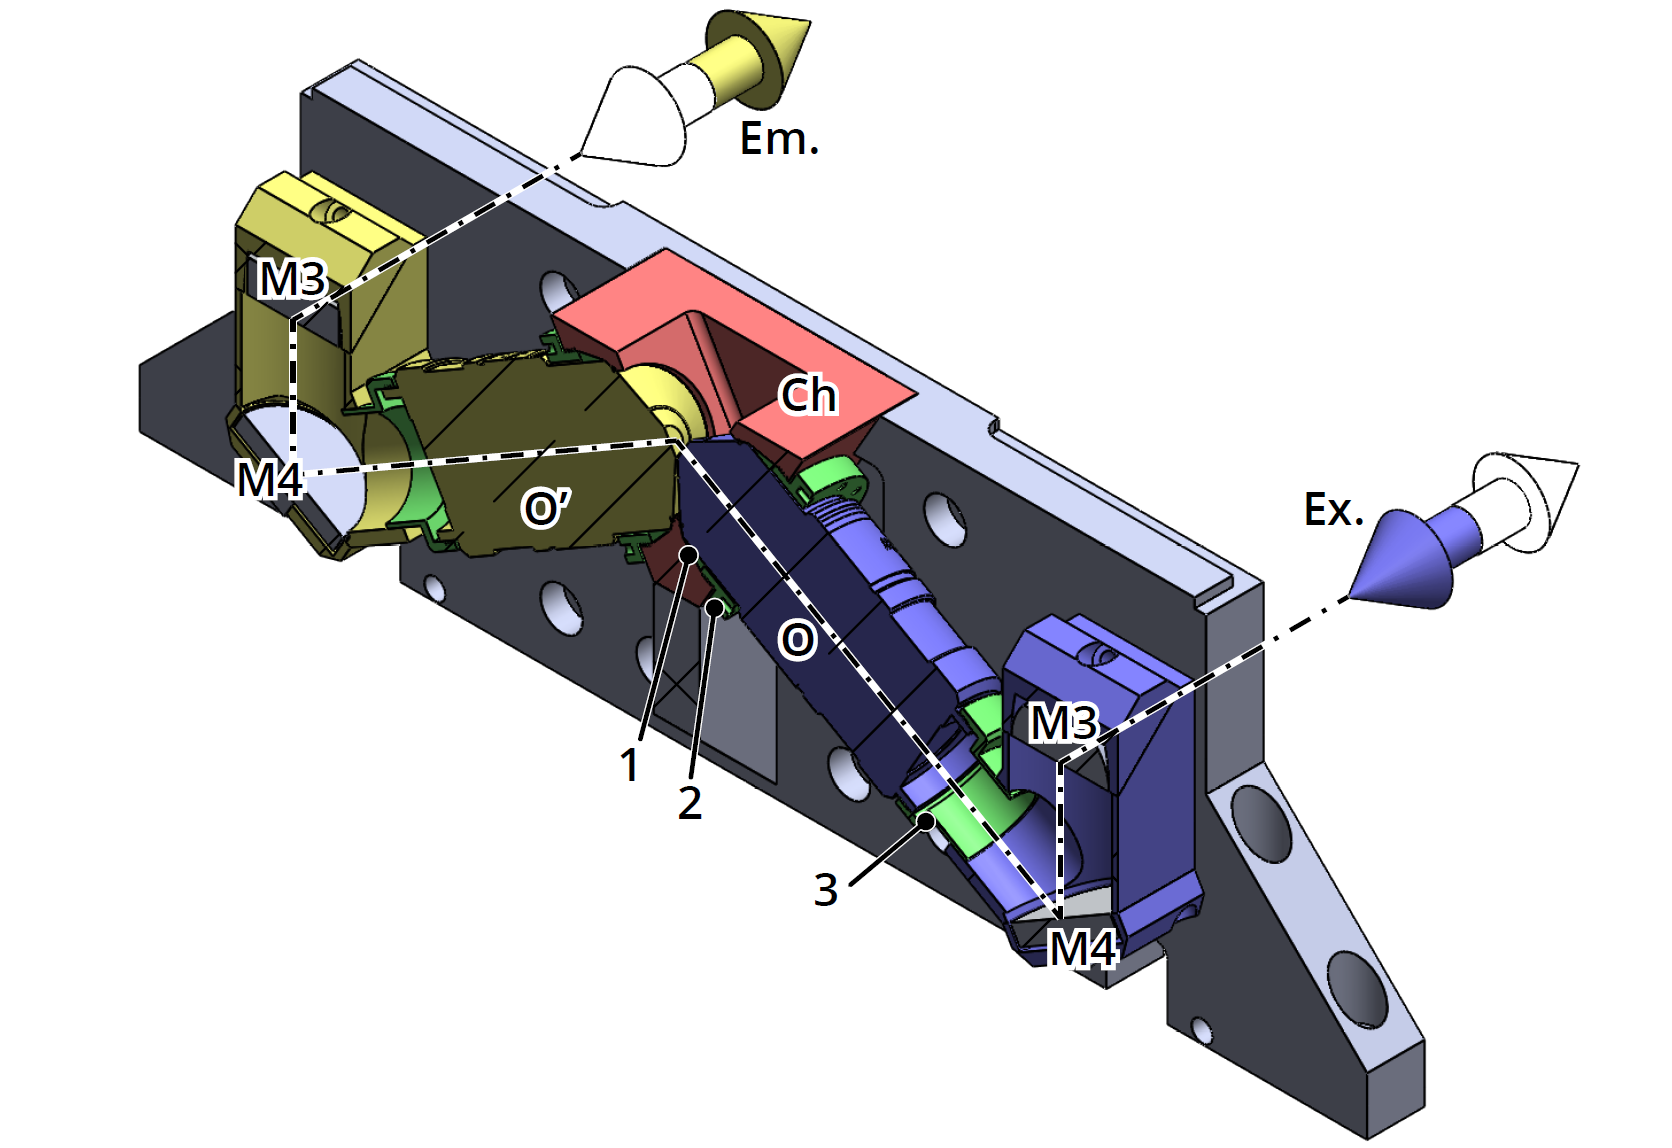
\includegraphics[width=0.8\textwidth]{SW/frontRender.png}
      \bcaption[The core unit of the microscope]{The two objectives (O and O') are mounted on a solid \SI{15}{mm} thick aluminium plate. Fitting on the objectives, a custom chamber (Ch) is holding the immersion medium for imaging. The mirror block with mirrors M3 and M4 directs the light to \SI{65}{mm} optical rails. Excitation (Ex.) and emission (Em.) light paths are indicated by the dash-dot line. Due to the symmetric arrangement, the excitation and illumination paths can be alternated. The objectives are secured with rings 1--3 (green, see main text for details).}
      \label{fig:Core}
    \end{figure}

    As the most important part of the microscope is actually the sample, the design is based around a core consisting of the imaging chamber and the objectives (\autoref{fig:Core}). Also part of the core are two mirror blocks placed at the back of the objectives, and three custom-designed rings to hold the objectives in place. The objectives are pointing slightly upwards, closing a \SI{60}{\degree} angle with the horizontal plane, and \SI{120}{\degree} angle with each other. 

    \subsubsection{Chamber}
    The chamber serves two purposes: it holds the immersion liquid necessary for imaging, and it keeps the objectives in the \SI{120}{\degree} position. The objectives are held by their necks as opposed to the standard mounting method, which is from the back, by the threads. The advantage of this is that any axial movements due to thermal expansion are greatly reduced, thus the focal plane position is more stable even when changing the imaging conditions.

    The chamber is machined from a high-performance plastic, polyether ether ketone (PEEK). This material has many beneficial properties: it is food safe, chemically highly inert, and resistant to most solvents used in a biology laboratory. Due to these properties, PEEK is live imaging compatible, even for sensitive samples, as it can also be autoclaved. Compared to other plastics its mechanical properties are also superior. It has high tensile and compressive strength, comparable to those of aluminium, low thermal expansion and low thermal conductivity. This can be beneficial when implementing temperature control, as thermal loss is reduced.

    The objectives are kept in place by two custom-designed rings (\autoref{fig:Core} 1, 2). The first ring has a cross sectional shape of a wedge, and sits tightly against both the objective and the wall of the chamber. The second ring can freely slide on the objective, and has threads matching the chamber. When turned in, the threaded ring pushes the wedge ring further in, which in turn presses against the objective and the chamber wall uniformly, thus preventing the objective from moving, and sealing the chamber at the same time. As the wedge ring is made from a soft plastic (delrin), it will press evenly against the objective preventing any damage. Given the conical shape of the ring, it will also automatically center the objective, ensuring correct positioning.

    To relieve any rotational stresses from the objective, the back of the objective is also supported  by the mirror block. This is not fixed, however. A third ring, made of PEEK is threaded on the objective, and slides into the opening of the mirror block. This reduces the forces on the objectives, while still allows for some movements that might occur in the axial direction due to thermal expansion.

    \subsubsection{Mirror blocks}
    \label{sec:mirrors}
    Apart from supporting the objectives from the back, the mirror blocks are housing two broadband dielectric mirrors (Thorlabs, BBE1-E03 and OptoSigma, TFMS-30C05-4/11) to direct the light to and from the objectives on a standard \SI{65}{mm} height, compatible with the Owis SYS65 rail system. The combination of two mirrors have two benefits compared to using just one. With a single mirror directly reflecting the light to the back, the entire assembly would need to be much higher to reach the desired \SI{65}{mm} height. This could result in stability problems. Furthermore, due to the \SI{60}{\degree} rotation angle of the objective, the image of the objective would also be rotated if using only a single mirror. With two mirrors the reflection planes can be kept orthogonal to the optical table, which will result in a straight image after the mirror block. This is not only beneficial when recording the images, but also when aligning the illumination arm. With the use of two mirrors, a convenient vertical scanning is required to produce the light-sheet; with a single mirror, the scanning direction would need to be rotated by \SI{60}{\degree}.


  
    \subsection{Illumination}

    The illumination arm of the microscope directs and shapes the laser beam to generate the proper light-sheet dimension at the sample. As was calculated in \autoref{sec:ls-design}, a beam diameter of \SI{1.2}{mm} is ideal for this setup.

    The illumination arm has three main roles:
    \begin{enumerate}
      \item expands the laser beam to the required size.
      \item images the galvanometric scanner to the back focal plane of the objective
      \item switches the laser light between the two objectives during imaging
    \end{enumerate}

    To achieve the desired beam diameter, a 1:2 beam expander (Sill Optics, 112751) is used in the reverse direction. As the output of the laser fiber produces a \SI{3}{mm} diameter beam, this will reduce it to \SI{1.5}{mm}. As this is already the required beam diameter, the lenses further in the illumination path will not introduce any magnification.
    
    % \subsubsection{Beam splitter unit}
    \label{sec:splitter}

    Switching between the two illumination arms is performed by a custom-designed beam splitter unit (\autoref{fig:splitter}). Instead of utilizing a 50/50 beam splitter cube and mechanical shutters, we exploit the fact that a galvanometric scanner is needed to generate the light-sheet. As this galvanometric scanner (Cambridge Technology, 6210B) has a relatively large movement range ($\pm \SI{20}{\degree}$) it is also suitable for diverting the beam from one illumination arm to the other.

    \begin{figure}[htb]
      \centering
      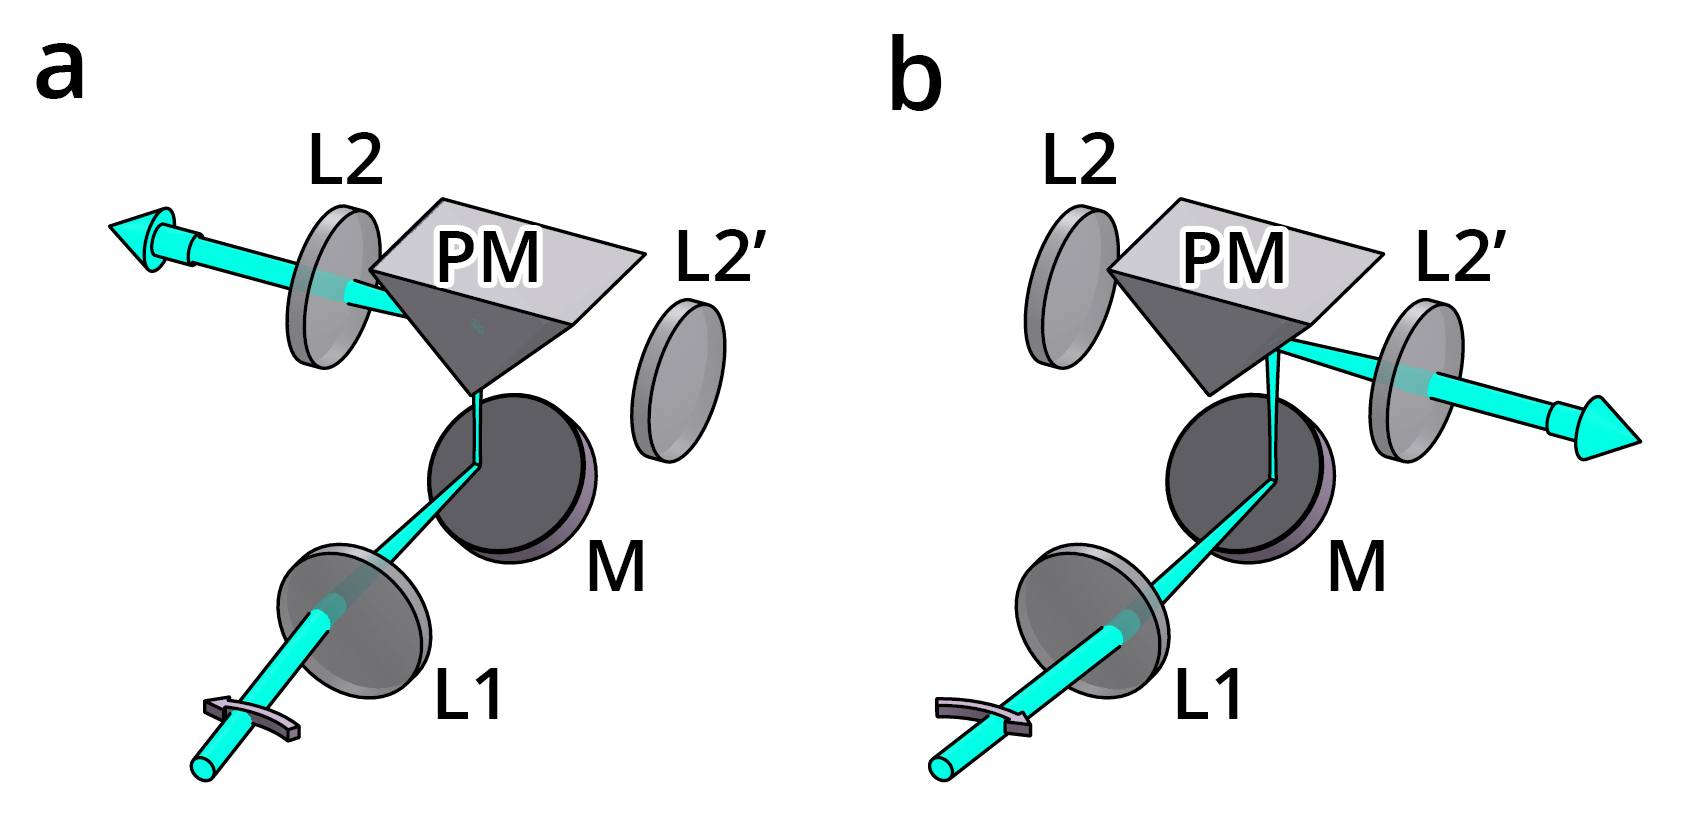
\includegraphics[width=0.8\textwidth]{SW/splitterFigure}
      \bcaption[Illumination branch splitting unit]{To divert the beam to either side, a right angle prism mirror is used in conjunction with a galvanometric scanning mirror. L1 acts as a scan lens, thus the beam is translated on mirror M. Depending on the scanner angle, the beam will be reflected either to the left (\textbf{a}) or to the right (\textbf{b}). L2 and L2' act as relay lenses, and will image the scanner movement to the corresponding intermediate planes.}
      \label{fig:splitter}
    \end{figure}

    Switching illumination side is done the following way. As the scanner is positioned at the focus of the first lens (L1, $f_1 = \SI{75}{mm}$, Edmund Optics, \#47-639), the rotational movement will result in a linear scanning movement on mirror M and the prism mirror PM (\autoref{fig:splitter}). Depending on the lateral position of the beam, it will hit either the left or the right leg of the prism (Thorlabs, MRAK25-E02), and will be reflected to either direction. As the galvanometric mirror can be precisely controlled through our custom software, we can set and save the position when the beam is centered on the left lens L2 ($f_2 = \SI{75}{mm}$, Edmund Optics, \#47-639) (\autoref{fig:splitter}a) and the position when the beam is centered on the right lens L2' (\autoref{fig:splitter}b). Lenses L1 and L2(L2') form a 1:1 relay system, and are imaging the scanner on mirror M1(M1') (\autoref{fig:fullSchematics}). This way we can use the same scanner to generate the light-sheet for both directions, depending on the initial offset position. This not only has the advantage of being able to electronically switch the illumination arms, but only requires a single galvanometric scanner instead of one for each arm.
    
    Due to the arrangement of the bottom mirror and the prism mirror the scanning direction will be rotated by \SI{90}{\degree}. This will result in a vertical scanning plane, which is exactly what we need to generate the light-sheet on the sample (see \autoref{sec:mirrors}).
    % \subsubsection{the rest of illumination}
    Further following the illumination path, two achromatic lenses L3 and L4 ($f_3 = f_4 = \SI{200}{mm}$) form a 1:1 relay, imaging the scanning axis to the back focal plane (BFP) of the objective.
    % To couple in the laser with the imaging path, a quad-band dichroic mirror (DM, Semrock, Di03-R405/488/561/635-t3-25x36) is used, matching the wavelengths of the laser combiner.

   

  \subsection{Detection}
    As the emitted light exits the objective and the mirror block, it is spectrally separated from the illumination laser light by a quad band dichroic mirror (DM, Semrock, Di03-R405/488/561/635-t3-25x36) matching the wavelengths of the laser combiner. The light is then focused by a \SI{400}{mm} achromatic lens (L5, Edmund Optics, \#49-281) onto the camera sensor (Andor Zyla 4.2 sCMOS). Just before the camera, a motorized filter wheel (FW, LEP 96A361) is placed to discriminate any unwanted wavelengths from the emission light. Although this is not in the infinity space, due to the very small angles after the \SI{400}{mm} tube lens, the maximum axial focal shift is $\sim \SI{50}{nm}$ only, which is negligible compared to the axial resolution of $\sim \SI{1.1}{\micro m}$.

    Similarly to the common scanner in the illumination path, the two detection arms share the same camera. Although two cameras could also be used, due to the operating principle of the microscope, the two objective are not used for imaging at the same time. This means a single camera is capable of acquiring all the images. However, the two distinct detection arms need to be merged to be able to use a single detector.
    
    Our solution to this problem is a custom-designed view-switching unit comprised of two broadband dielectric elliptical mirrors (Thorlabs,BBE1-E03) facing opposite directions, mounted on a high precision linear rail (OptoSigma, IPWS-F3090). Depending on the rail position, either the left (\autoref{fig:dualMirror}a) or the right (\autoref{fig:dualMirror}b) detection path will be reflected upwards, to the camera. 

    Moving the switcher unit is performed by a small, \SI{10}{mm} diameter pneumatic cylinder (Airtac, HM-10-040) that is actuated by an electronically switchable 5/2 way solenoid valve (Airtac, M-20-510-HN). This solution offers a very fast switching between views, up to \SI{5}{Hz}, depending on the pressure, and it is extremely simple to control, as only a digital signal is necessary to switch the valve. 

      \label{sec:dualMirror}
      \begin{figure}[tb]
        \centering
        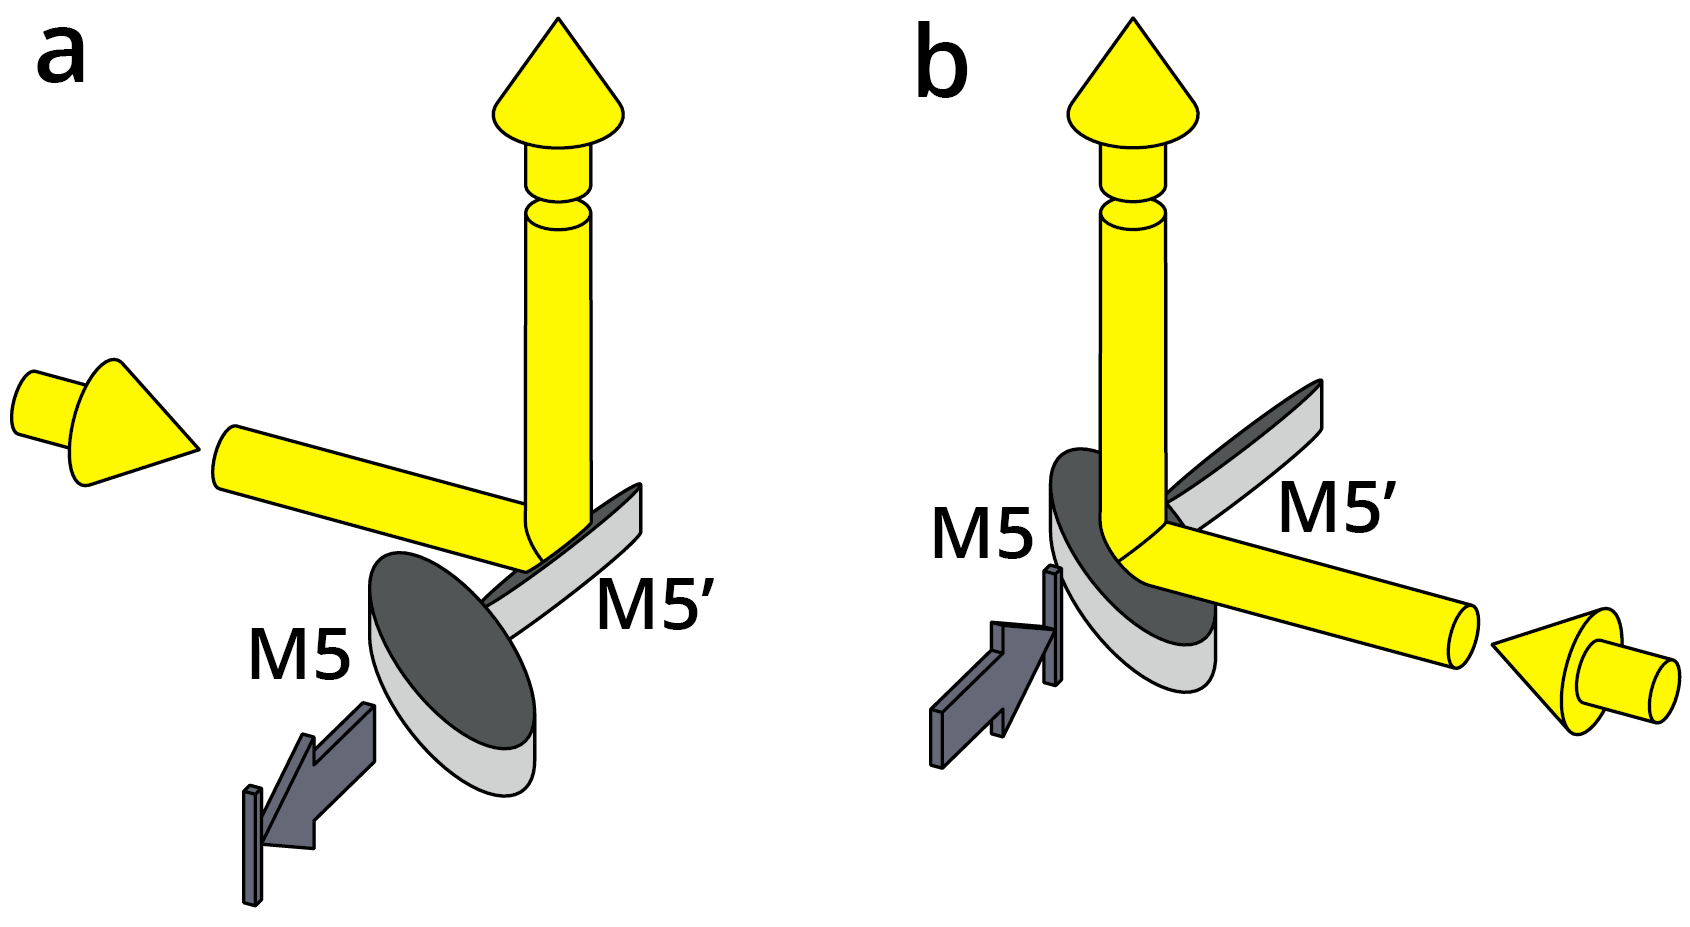
\includegraphics[width=0.8\textwidth]{SW/dualMirrorFigure}
        \bcaption[Detection branch switching unit]{To be able to image both views on the same camera, a moveable mirror unit is introduced. Depending on the imaging direction, the mirror block is either moved backward (\textbf{a}) or forward (\textbf{b}) to reflect the light up to the camera. Since the movement is parallel to the mirrors' surfaces, the image position on the sensor is not dependent on the exact position of the mirrors.}
        \label{fig:dualMirror}
      \end{figure}
        
      


     %##    ##       ####  ######   ##    ## 
    %# ##   ##        ##  ##    ##  ###   ## 
   %#   ##  ##        ##  ##        ####  ## 
  %#     ## ##        ##  ##   #### ## ## ## 
  %######## ##        ##  ##    ##  ##  #### 
  %#     ## ##        ##  ##    ##  ##   ### 
  %#     ## ######## ####  ######   ##    ## 
\section{Optical alignment}
  Precise alignment of the illumination and detection paths are crucial for high quality imaging, and has a pronounced importance for high magnification and high resolution optical systems. 
  Due to the symmetrical setup of the microscope, we will only describe the alignment of one side, as the same procedure is also applicable to the other side. References to optical components will be as defined in \autoref{fig:fullSchematics}.

  \subsection{Alignment of the illumination branches}

    The two illumination branches start with a common light source, a single-mode fiber coupled to a laser combiner, and they also share a galvanometric mirror that performs the beam scanning to generate the virtual light-sheet. Likewise shared is a scan lens focusing on the galvanometric mirror (GM), and the illumination splitter unit (PM, see section \ref{sec:splitter}).

    Alignment of the illumination arms is done in three steps. First the laser beam is aligned on the rail that holds the scanner, lens L1, and the splitter unit PM. This is performed by two kinematic mirrors placed between the fiber output and the galvanometric mirror (not shown on figure). Using these two mirrors it is possible to freely align the beam along all four degrees of freedom: translation in two orthogonal directions and rotation around two orthogonal axes. Beam alignment on the rail is tested by using two irises at the two ends of the rail, if the beam passes through both of them we consider it centered and straight on the optical axis.

    After the beam is aligned on the first rail, lens L1 and the splitter unit PM are placed in the measured positions to image the galvanometric mirror on mirror M1 using lenses L1 and L2. Correct positioning of the splitter unit along the rail is crucial, since this will affect the lateral position and tilt of the beam exiting the unit. To some extent this can also be compensated by adjusting the two mirrors before the galvanometric mirror, but should be avoided if possible as this will also displace the beam from the center of the galvanometric mirror.

    After the initial alignment of the illumination arms, when the laser is already coupled into the objective, the fine adjustments are performed based on the image of the beam through the other objective. The beam is visualized by filling the chamber with a 0.1\% methylene blue solution. As this solution is fluorescent and can be excited in a very large range, it is well suited to visualize the beam during adjustment.

    \paragraph{Adjusting beam position}
      Beam position can be adjusted by either translating the beam in a conjugated image plane (I'), or by rotating the beam in a conjugated back focal plane (BFP'). The setup was designed in a way that BFP' coincides with mirror M1. This mirror is mounted in a gimbal mirror mount, allowing to rotate the mirror exactly around its center, which avoids unwanted translational movements, and results in pure rotation of the beam. Lens L3 is positioned exactly 1 focal length away from the mirror, thus acting as a scan lens, and transforming the rotational movements to translation. This translation is further imaged and demagnified by the tube lens L4 and the objective O onto the sample.


    \paragraph{Adjusting beam tilt}
      Beam tilt can be adjusted by either rotating the beam in an intermediate image plane (I'), or translating it at the back focal plane (BFP). As mirror M2 is relatively far from the back focal plane, adjusting it will mostly result in translation that will rotate the beam in the image plane. This movement, however, will also introduce translations, and has to be compensated by adjusting mirror M1. The light-sheet needs to be tilted by \SI{30}{\degree} to coincide with the focal plane of the other objective, but this level of adjustment is not possible with M2. In order to allow for a pure rotation of the light-sheet, we mounted the dichroic mirrors on linear stages (OptoSigma, TSDH-251C). By translating the dichroic mirror, the illumination laser beam gets translated at the back focal plane, which will result in a pure rotational movement at the sample. Coarse alignment of the light-sheet is performed by adjusting the dichroic position while inspecting the light-sheet through a glass window in the chamber. Precise alignment is done afterwards based on the image of the beam visualized in a fluorescent medium.


    % \paragraph{Adjusting beam axial position.}


    \paragraph{Adjusting the scanning-plane angle}
      After the beam is properly aligned, \textit{i.e.}, it is in focus and in the center of field of view, it is still necessary to check if the scanning direction is parallel to the imaging plane. It is possible that the beam is in focus in the center position, but when moved vertically it drifts out of focus due to a tilted scanning angle. This tilt can be compensated by mirror M1, which is placed at the conjugate back focal plane BFP'. Between lenses L3 and L4 a magnified version of the light-sheet will be visible, and the tilt can be checked by placing an alignment target in the optical path while scanning the beam. By tilting mirror M1 up or down the scanning pattern not only translates, but it also rotates if the mirror surface is not exactly vertical. Since M1 and GM are in conjugated planes, the tilt and offset can be performed independently. The tilt is first fixed by M1 while inspecting the target, and the beam is re-centered by changing the offset on the galvanometric mirror. Moving the galvanometric mirror will not introduce tilt, since in this case rotation axis is perpendicular to the reflection plane.




  \subsection{Alignment of the detection branches}
    Since the detection path is equivalent to a wide-field detection scheme, its alignment is much simpler than that of the illumination branches. The only difference is the detection branch merging unit (see \autoref{sec:dualMirror}.) which features two moving mirrors. This, however, does not affect the alignment procedure, since the movement direction is parallel to both mirrors' surfaces, meaning that the exact position of the mirrors will not affect the image quality, as long as the mirrors are not clipping the image itself. A stability test was performed to confirm the consistent switching performance of the mirror unit before the final alignment took place (see \autoref{sec:mirrorStability}).

    % TODO: complete paragraph
    % The final alignment procedure 

    \paragraph{Positioning the tube lens}
      The position of the tube lens determines the focal plane that is being imaged on the camera sensor. Ideally, the tube lens's distance from the camera sensor is exactly the tube lens's focal length, which will ensure the best imaging performance. If the tube lens's distance is not correct, the focal plane will be slightly shifted in the axial direction. Small shifts will not necessarily have detrimental effect on the image quality, because the light-sheet can also be shifted accordingly. Because of the shifted focal and image planes, however, the magnification of the system will be affected, and will change depending on the amount of defocus. For this reason we aim for positioning the tube lens as close to the theoretical position as possible.

      Our tube lens is a compound, achromatic lens with a center thickness of \SI{12.5}{mm}, and edge thickness of \SI{11.3}{mm}. Its effective focal length is \SI{400}{mm} which will produce a 50x magnified image. The back focal length is \SI{394.33}{mm} which we measured from the camera chip, and the lens was positioned at this theoretically optimal position.

    \paragraph{Adjusting the correction collar}
      The Nikon 25x objectives used for this setup have a built in correction ring that can be used to correct spherical aberrations resulting from refractive index differences when imaging samples behind a coverslip. This can be also effectively used to correct for any spherical aberrations occurring from imaging through the FEP foil. Although these aberrations are expected to be extremely low, due to the relatively thin, \SI{50}{\micro m} foil thickness, and the close matching of refractive index ($n_{\mathrm{FEP}} = 1.344$, $n_{\mathrm{H_2O}}=1.333$), for optimal, aberration free image quality it can not be neglected.

      The correction collars are adjusted by inspecting a gel-suspended fluorescent bead specimen with the microscope, where the beads can act as a reporter of the point spread function of the microscope. The alignment can be performed ``live" by inspecting the bead image quality for aberrations. By gradually changing the correction collar, the ring artifacts are minimized on out-of-focus beads, and the peak intensity is maximized for in-focus beads. By moving the correction ring, the focal plane is also slightly shifted, which has to be compensated by shifting the light-sheet correspondingly to coincide with the correct imaging plane.

    \paragraph{Adjusting the field of view}
      To allow for proper sampling of the image, we use 50\texttimes\ magnification, which combined with the \SI{6.5}{\micro m} pixel pitch of our sCMOS camera, will result in a \SI{0.13}{\micro m} pixel size. The full field of view recorded by the camera is $2048 \times \SI{0.13}{\micro m} = \SI{266.24}{\micro m}$.
      % The full field of view the objective provide, are larger than this at \SI{800}{\micro m}.
      To ensure the best image quality, we align the center of the objective field of view on the camera sensor, since this region has the best optical properties in terms of numerical aperture, aberration correction and flatness of field.

      Field of view alignment can be performed by using mirror M5 just before the detection merging unit. To identify the center region of the field of view, diffuse white light is used to illuminate the entire sample chamber, and it is imaged on the camera. Then, mirror M5 is adjusted until the top edge of the field of view becomes visible, \textit{i.e.}, where the illumination from the chamber is clipped. This will have a circular shape. Afterwards, adjusting the mirror in the orthogonal direction, the left-right position of the field of view can be adjusted, by centering the visible arc on the camera sensor.

      After the horizontal direction is centered, vertical centering is performed. This, however can not be centered the same way as the horizontal direction, since for that we would have to misalign the already aligned horizontal position. To determine the center, we move the field of view from the topmost position to the bottom. During this process the number of  turns of the adjustment screw is counted (this can be done accurately by using a hex key). After reaching the far end of the field of view, the mirror movement is reversed, and the screw is turned halfway to reach the middle.







\section{Control unit}

  The microscope's control and automation is performed by an in-house designed modular microscope control system developed in LabVIEW \cite{balazs_development_2013}. The core of the system is a National Instruments cRIO-9068 embedded system that features an ARM Cortex A9 processor and a Xilinx Zynq 7020 FPGA.
  Having both chips in the same device is a great advantage, since the main processor can be used to run most of the microscope control software, while the FPGA can be used to generate the necessary output signals in real time and with high precision.
  
  The embedded system is complemented by a high-performance workstation that is used to display the user interface of the microscope, and to record the images of the high-speed sCMOS camera. 

  \subsection{Hardware}
    Various components need to be synchronized with high precision to operate the microscope: a laser combiner to illuminate the sample; a galvanometric scanner to generate the light-sheet; stages to move the samples; filter wheel to select the imaging wavelengths; and a camera to detect the fluorescence signal.    
    % For more details on the exact models, see Appendix \ref{sec:BOM}.
    For high speed image acquisition, all of these devices have to be precisely synchronized in the millisecond range, and some even in the microsecond range.
    Although they require different signals to control them, we can split them into three main categories:

    \begin{center}
      \begin{tabular}{lll}
        \textbf{digital input} & \textbf{analog input}   & \textbf{serial communication} \\ \hline
        camera exposure    & galvanometric position & filter wheel         \\
        laser on/off (\texttimes 3) & laser intensity (\texttimes 3) & stages (\texttimes 2)
      \end{tabular}
    \end{center}

    All devices are connected to the NI cRIO 9068 embedded system, either to the built in RS232 serial port, or to the digital and analog outputs implemented by C-series expansion modules (NI 9401, NI 9263, NI 9264). The workstation with the user interface is communicating with the embedded system through the network. The only device with a connection to both systems is the camera: the embedded system triggers the image acquisition, and the images are piped to the workstation through a dual CameraLink interface, capable of a sustained \SI{800}{MB/s} data transfer rate (\autoref{fig:HW}).

    \begin{figure}
      \centering
      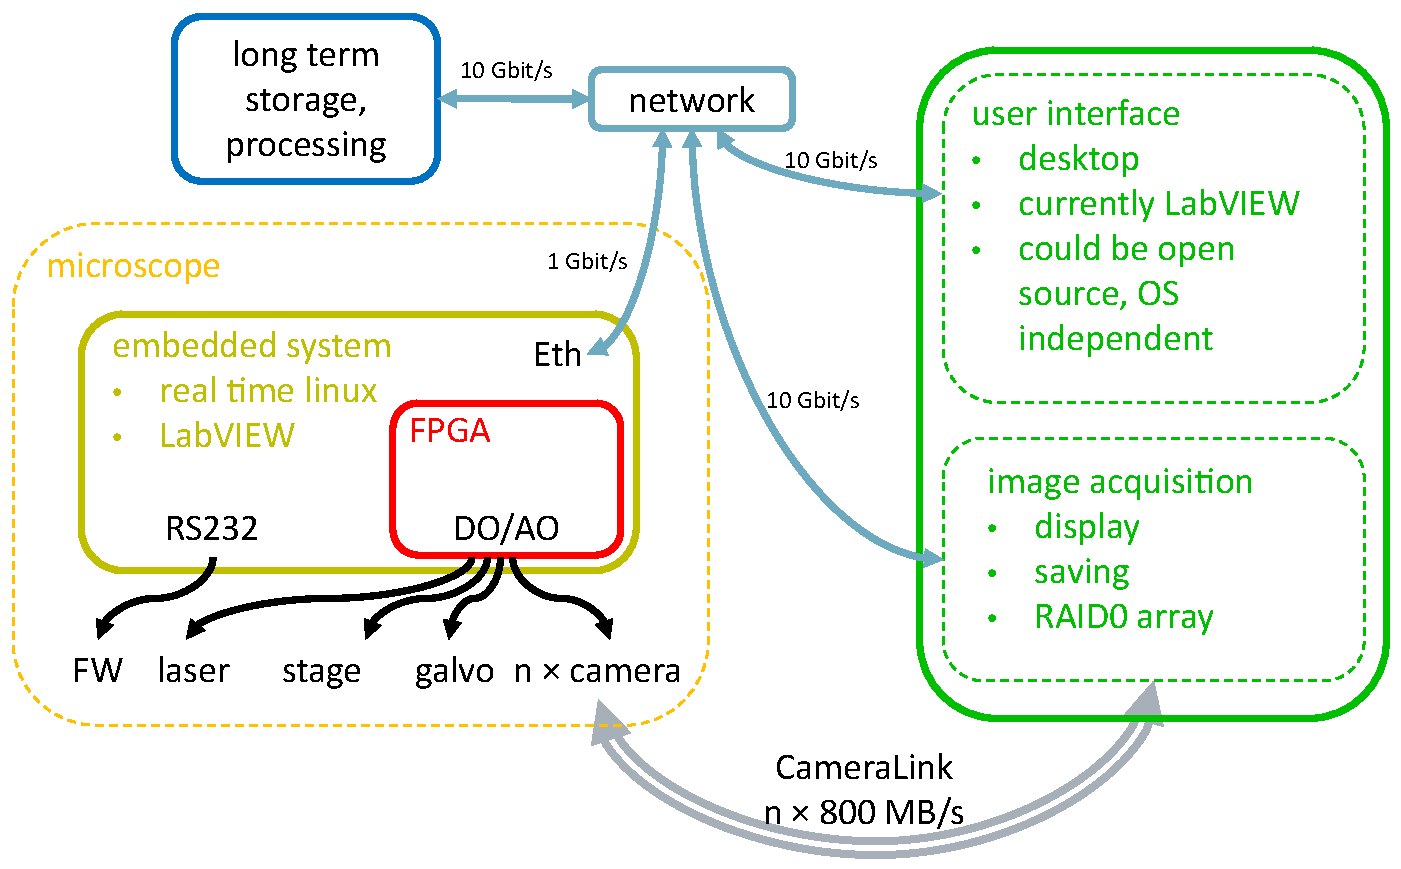
\includegraphics[width=0.9\textwidth]{HW}
      \bcaption[Microscope control hardware and software architecture]{The embedded system responsible for the hardware control and the workstation are communicating through the network using the WebSocket protocol. The electronic devices of the microscope are either controlled through digital/analog signals, or through serial communication. The camera is also connected to the workstation with a CameraLink connection, which transmits the recorded images.}
      \label{fig:HW}
    \end{figure}
  
  \subsection{Software}
    \label{sec:software}

    \begin{figure}
      \centering
      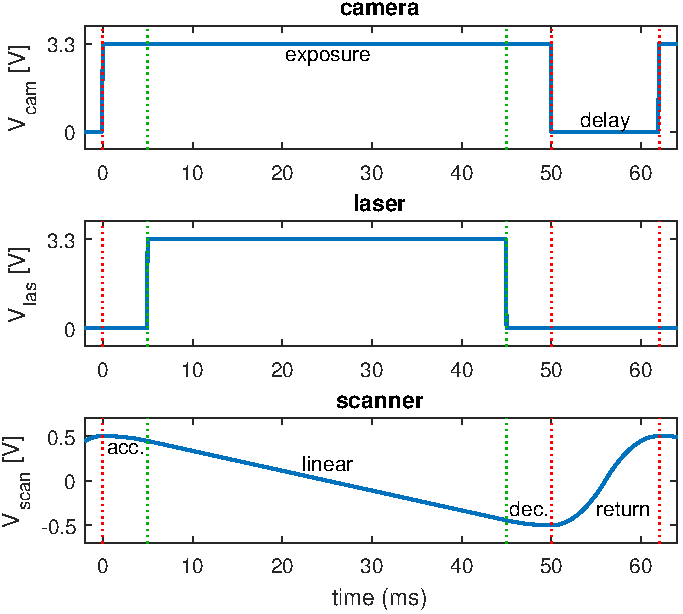
\includegraphics[width = 0.6\textwidth]{fpgaTraces_scanner}
      \bcaption[Digital and analog control signals]{Example traces for recording a single plane with \SI{50}{ms} exposure time and \SI{12}{ms} delay. During the exposure of the camera the scanner has 3 sections: acceleration (acc.), linear, and deceleration (dec.). The laser line is synchronized with the scanner linear section to ensure even illumination. }
      \label{fig:traces}
    \end{figure}

    Being able to precisely control all of the instruments not only relies on the selected hardware, but just as much on the software. Our custom software is developed in LabVIEW, using an object-oriented approach with the Actor Framework. The embedded system is responsible for the low-level hardware control, for keeping track of the state of all devices, saving the user configurations, and automating and scheduling the experiments. It also offers a Javascript Object Notation (JSON) based application programming interface (API) through WebSocket communication. This is mainly used to communicate with the user interface, however it also offers the possibility of automated control by an external software.

    \subsubsection{FPGA software}
      The on-board FPGA is responsible for generating the digital and analog output signals based on the microscope settings (\autoref{fig:traces}). To avoid having to calculate all the traces for a whole stack, the main software only calculates a few key parameters of the traces that are necessary to completely describe them. The FPGA then calculates the signals in real time, and outputs them with microsecond precision.

      To describe the traces, we define them as a concatenation of \textit{sections}. Each section has 3 or 5 parameters, depending on whether they are digital or analog. Both types have three common properties: \texttt{value}, \texttt{length}, and \texttt{type}. The analog sections additionally contain a \texttt{dValue} and a \texttt{ddValue} element describing the velocity and the acceleration of the signal. This allows us to generate piecewise functions made of second-order polynomials.

      The \texttt{type} element contains information on which value should be updated for the current section. Setting the lowest bit high will update the \texttt{value}, setting the second bit high will update the \texttt{dValue}, and setting the third bit high will update the \texttt{ddValue}. This feature allows to define smooth transitions between the sections, and also to define more complex signals, as long as they are periodic in the second derivative.


    %#######  ########  ######  ##     ## ##       ########  ######  
    %#     ## ##       ##    ## ##     ## ##          ##    ##    ## 
    %#     ## ##       ##       ##     ## ##          ##    ##       
    %#######  ######    ######  ##     ## ##          ##     ######  
    %#   ##   ##             ## ##     ## ##          ##          ## 
    %#    ##  ##       ##    ## ##     ## ##          ##    ##    ## 
    %#     ## ########  ######   #######  ########    ##     ######  

%\section{Validating the system}

\section{Validating and characterizing the microscope}
  \begin{figure}
    \begin{subfigure}[t]{0.5\textwidth}
      \centering
      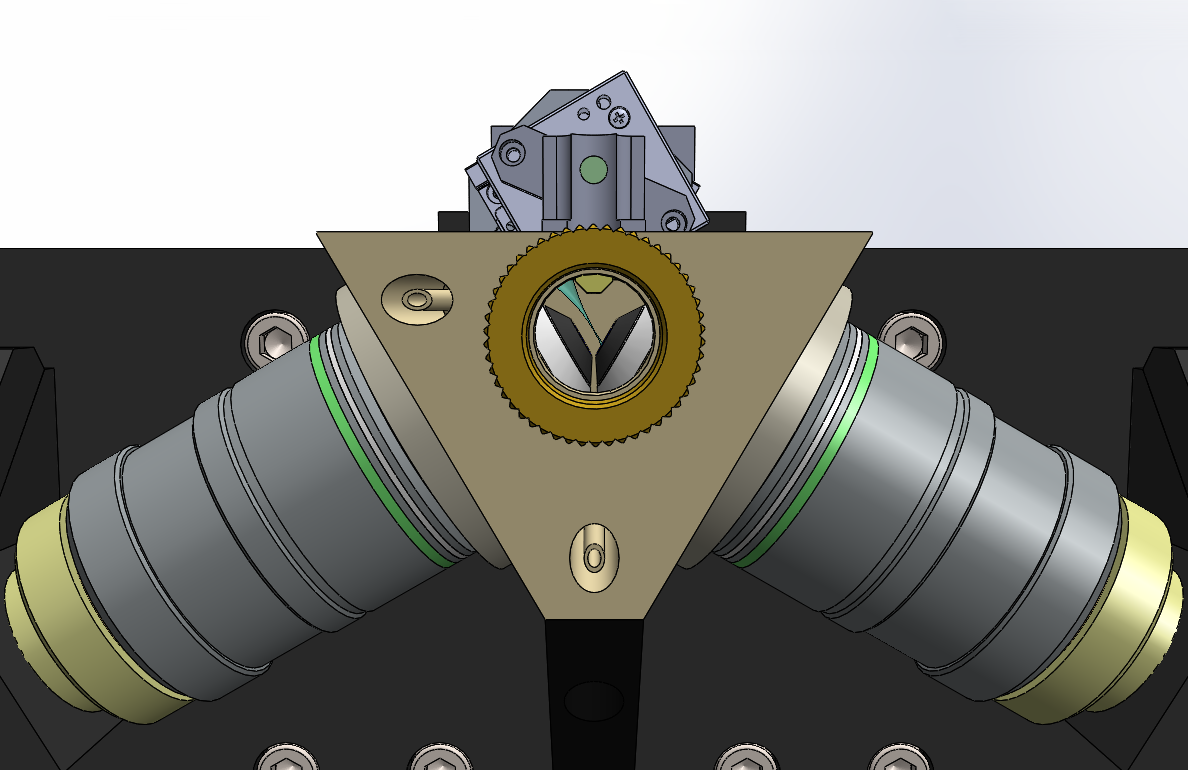
\includegraphics[width=\textwidth]{photos/front_solidworks_overlay}
      \caption{Front view of the SolidWorks design.}
    \end{subfigure}
    \begin{subfigure}[t]{0.5\textwidth}
      \centering
      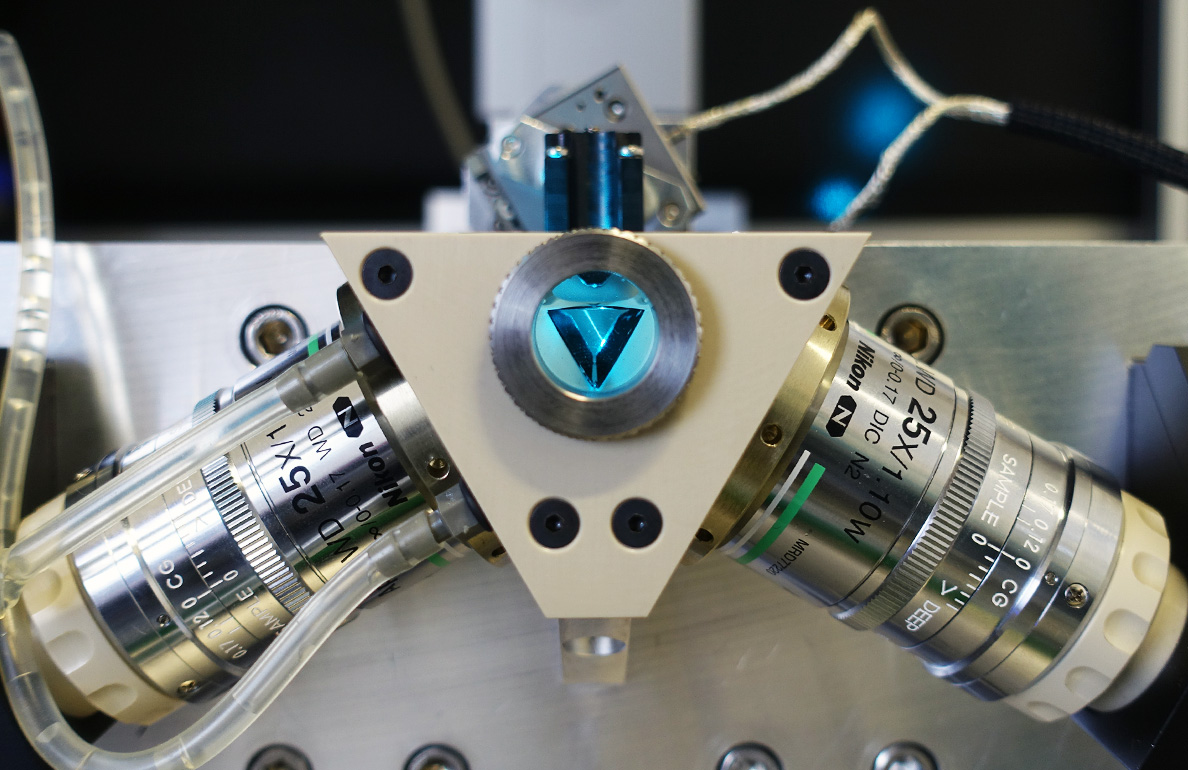
\includegraphics[width=\textwidth]{photos/front_photo_overlay.jpg}
      \caption{Front view of the microscope.}
    \end{subfigure}
    \\
    \begin{subfigure}[t]{1\textwidth}
      \centering
      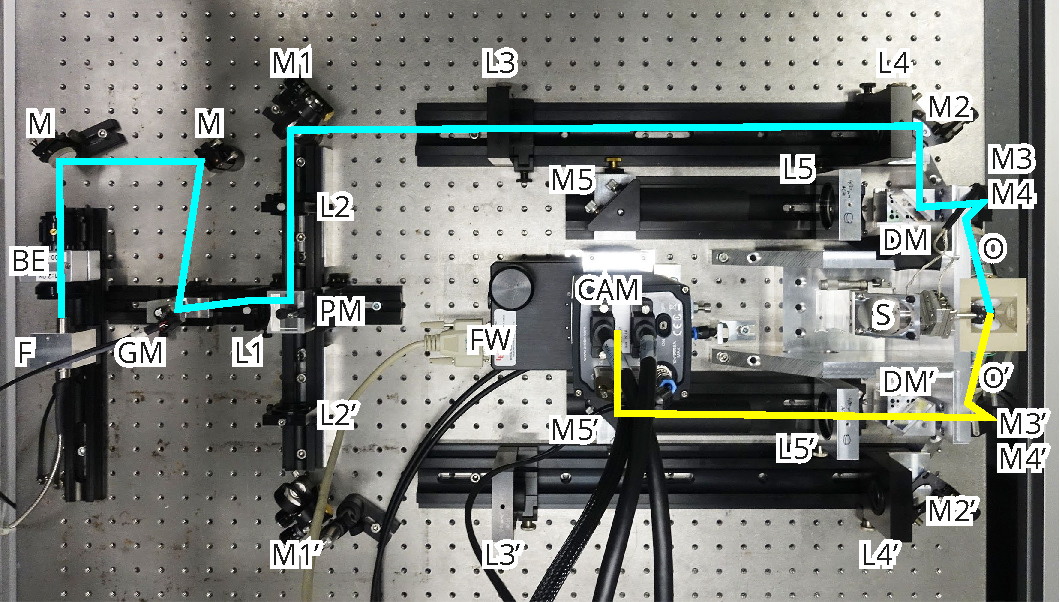
\includegraphics[width=\textwidth]{photos/top+light}
      \caption{Top view of the microscope.}
    \end{subfigure}
    \bcaption[Completed DualMouse-SPIM]{The excitation and emission light paths are depicted with blue and yellow lines respectively. Component numbering corresponds to \autoref{fig:fullSchematics}. Detection branch merging unit, and mirrors M6 and M6' are underneath the camera and filter wheel. BE -- beam expander, CAM -- camera, DM -- dichroic mirror, F -- fiber, FW -- filter wheel, L -- lens, M -- mirror, O -- objective, PM -- prism mirror, S -- stage}
    \label{fig:frontView}
  \end{figure}

  % Resolution for Lattice light-sheet \cite{chen_lattice_2014}: \SI{230}{nm} in x and \SI{370}{nm} in z
  % \cite{chhetri_whole-animal_2015}

  Following the design phase, all custom parts were manufactured by the EMBL mechanical workshop, and the microscope was assembled on a MellesGriot optical table (\autoref{fig:frontView} and \autoref{fig:3D}). The microscope was equipped with an Andor Zyla 4.2 sCMOS camera that offers a large field of view of 2048\texttimes 2048 pixels with a pixel pitch of \SI{6.5}{\micro m}. It offers a high dynamic range of 1:30,000, and high frame rate at 100 frames per second (fps), while readout noise is minimal (0.9 e$^-$).
  
  To evaluate the performance of the microscope, we conducted various measurements, concerning the stability and the resolution of the system. The methods and results of these measurements will be presented in this section.

  \subsection{Methods}

  \label{sec:methods2}

  \subsubsection{Preparation of fluorescent bead samples}
    \label{sec:beads}
    For registration and resolution measurements we used TetraSpeck \SI{0.5}{\micro m} diameter fluorescently labeled beads (ThermoFisher, T7281). The stock bead solution was thoroughly vortexed and sonicated for \SI{5}{min} before diluting it 1:100 in distilled water. The diluted bead solution was stored at \SI{4}{\degree C} until use. GelRite (Sigma-Aldrich, G1910) gel was prepared in distilled water at 0.8\% concentration with 0.1\% $\mathrm{MgSO_4\cdot 7 H_2O}$ and kept at \SI{70}{\degree C} until use. \SI{50}{\micro l} of the diluted bead solution was added with a heated pipette tip to \SI{450}{\micro l} of gel solution at \SI{70}{\degree} to prevent  polymerization. The gel was thoroughly vortexed, and loaded to glass micropipettes (Brand \SI{100}{\micro l}). The gel was allowed to cool to room temperature and stored in a petri dish under $\mathrm{dH_2O}$ at \SI{4}{\degree C} until use. For imaging a small piece of gel was extruded from the capillary, cut off, and placed in the sample holder. After positioning the gel to the bottom of the sample holder, the holder was filled with \SI{200}{\micro l} $\mathrm{dH_2O}$.

  \subsubsection{Preparing the sample holder}
    The sample holder was lined with \SI{12.5}{\micro m} (PSF measurements) or \SI{50}{\micro m} (mouse zygote and \textit{Drosophila} embryo imaging) thin FEP foil (Lohmann, RD-FEP050A-610). The FEP foils were cut to size, washed with 70\% ethanol followed by a second wash with $\mathrm{dH_2O}$. After washing, both surfaces of the foils were chemically activated by a \SI{20}{s} plasma treatment (PlasmaPrep2, Gala Instrumente). The foils were then stored in a petri dish until further use, separated by lens cleaning tissues (Whatman, 2105-841). Before imaging, the sample holder was cleaned with dish soap, rinsed with tap water, rinsed with 70\% ethanol, and rinsed with $\mathrm{dH_2O}$. The prepared foils were glued to the inside of the cleaned sample holder with medical grade silicon glue (twinsil speed, picodent). During the \SI{5}{min} curing process the foil was pressed against the sample holder by a custom made press fitting the shape of the sample holder. Final dilution of the stock bead solution in the gel is 1:1000.

  \subsubsection{Drosophila embryo imaging}
    \textit{Drosophila melanogaster} embryos (fly stock AH1) expressing fluorescent nuclear (H2A-mCherry) and centriole (ASL-YFP) markers were collected on apple juice agar plates and dechorionated in 50\% bleach solution for \SI{1}{min}. After rinsing the bleach with deionized water, the embryos were placed in the sample holder under PBS solution. A small piece of gel containing fluorescent beads were also placed next to the samples to aid in multi-view registration.

  \subsubsection{Mouse zygote imaging}
    Fixed mouse zygotes labeled with Alexa Fluor 488 (microtubules) and Alexa Fluor 647 (kinetochores) coupled secondary antibodies were kindly provided by Judith Reichmann. Zygotes were transferred to the sample holder, and imaged in PBS. To allow for multi-view reconstruction, a small piece of gel containing fluorescent beads was placed next to the zygote in the sample holder. After imaging the zygote from both views, the beads were also recorded using the same stack definitions. After data acquisition, the multi-view datasets were registered and deconvolved in Fiji \cite{schindelin_fiji:_2012} using the Multiview Reconstruction Plugin \cite{preibisch_software_2010,preibisch_efficient_2014}. The deconvolution was based on a simulated PSF generated in Fiji with the PSF Generator plugin \cite{kirshner_3d_2011} using the Born-Wolf PSF model \autoref{sec:psf-simu}. $\mathrm{NA_{ex}}=0.1$, $\mathrm{NA_{em}}=1.1$, n=1.33, $\lambda_{ex} = \SI{488}{nm}$, $\lambda_{em} = \SI{510}{nm}$.

\subsection{Results}

  \subsubsection{Stability of the view switcher unit}
    \label{sec:mirrorStability}

    \begin{figure}
      \centering
      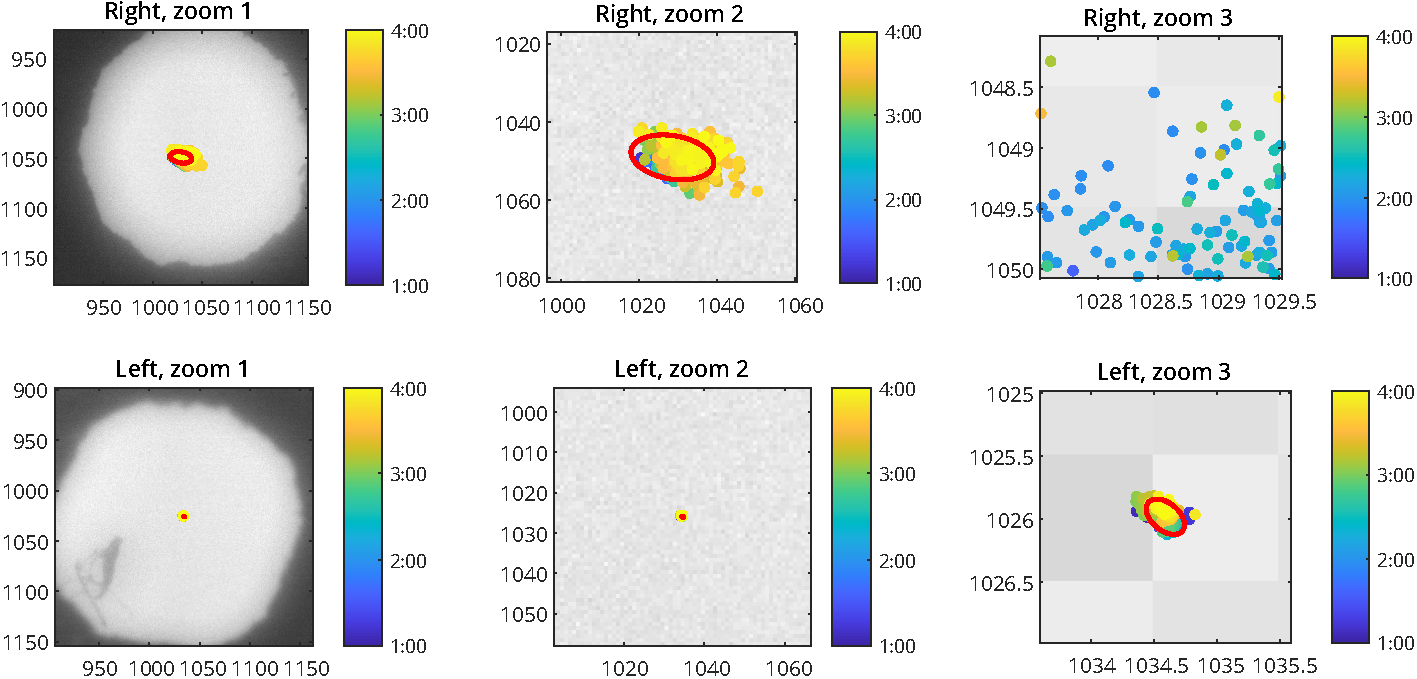
\includegraphics[width=\textwidth]{trackCenter}
      \bcaption[Stability measurements of view switcher unit] {A closed aperture was imaged on the camera from both views, every \SI{10}{s}, for \SI{4}{h}. The dots represent the center of each frame, color coded with the time. The red ellipse represents the 95\% confidence interval of the measured positions based on principal component analysis. Standard deviations for right view: $\sigma_1 = \SI{4.37}{px}$, $\sigma_2 = \SI{2.26}{px}$; for left view: $\sigma_1 = \SI{0.07}{px}$, $\sigma_2 = \SI{0.04}{px}$.}
      \label{fig:stability}
    \end{figure}

    As the view switcher unit is a custom-designed solution for this microscope, it is necessary to evaluate the effect of the switching on the field of view. Given that this is a moving unit, many mechanical imprecisions can introduce a drift in the final image. 

    To assess the reproducibility in the movement of the detection branch switching unit, a long-term stability test was conducted. To exclude all other factors (such as sample drift), we imaged the opening of two closed irises that were mounted on the detection optical rail. Image formation was done by two achromatic lenses ($f=\SI{75}{mm}$) positioned directly after mirrors M5 and M5'.
    
    The apertures were imaged from both views every 10 seconds, for \SI{4}{h}, for a total of 1440 images per view, and 2880 switches. The center of the aperture was segmented on all images using Matlab, and tracked to assess any drift occurring during the \SI{4}{h} time lapse (\autoref{fig:stability}). To visualize the uncertainty of the aperture's position, we performed principal component analysis (PCA) on the positions and visualized the results by plotting the 95\% confidence ellipse on the images. Although the right view had a significant spread with a standard deviation of \SI{4.37}{px} and \SI{2.26}px along the long and short axes respectively, the left view was extremely stable, and the standard deviation was only \SI{0.07}{px} and \SI{0.04}{px} for the long and short axes respectively. This result implies that there is no conceptual limitation in reaching sub-pixel reproducibility with the view switching unit, although some optimization is still needed for the right view to reach the same stability as the left view.

    

  \subsubsection{Characterizing the illumination profile}

    \begin{figure}[bthp]
      \centering
      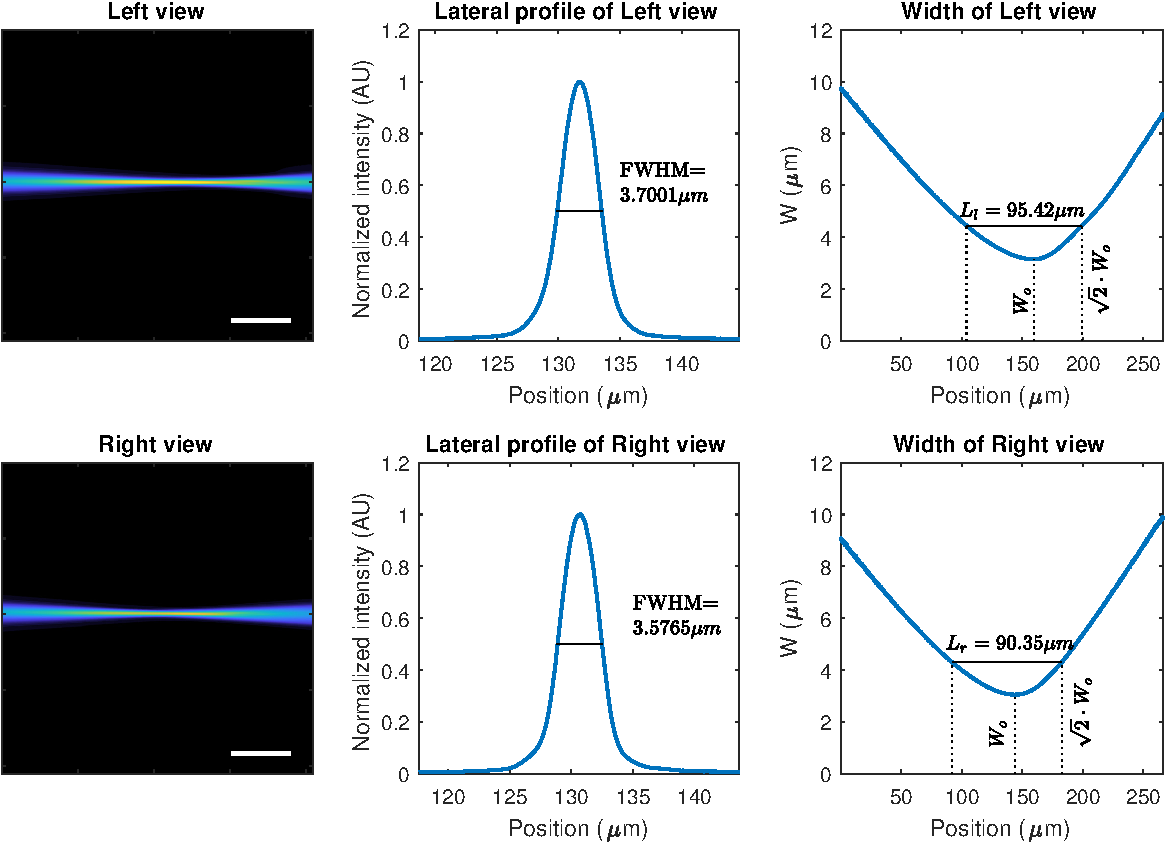
\includegraphics[width=\textwidth]{beamPlots_view.pdf}
      \bcaption[Illumination beam profile]{Average of 500 stationary beam images for both left (top left) and right objectives (bottom left). Beam intensity profile along the waist of each beam is plotted in the center column. The right column shows the beam width profile of each beam ($1/e^2$). Scale bar, \SI{50}{\micro m}.}
      \label{fig:beamProfiles}
    \end{figure}

    Since a Gaussian beam is used for illumination, its intensity profile depends on the axial position (\autoref{eq:gaussian}). Although the total intensity at any cross section of the beam is constant, the peak intensity varies due to the diverging beam. To assess any non-uniformities in the illumination pattern, we measured the illumination beam intensity for each view.

    To visualize the beam, the chamber was filled with a fluorescent solution (0.1 \% methylene blue in distilled water). In order to increase the signal-to-noise ratio of these images, a long exposure time of \SI{200}{ms} was used, and 500 images of each beam were averaged. Background images were acquired by repeating the image acquisition with the laser turned off. The average of the background images were subtracted from the averaged beam images, resulting in the beam intensity profile (\autoref{fig:beamProfiles}).

    To determine the beam waist position we measured the beam thickness (FWHM) for each column of the averaged images, and located the position of the minimal width. The beam width at the waist position for the left view was   \SI{3.70}{\micro m}, and for the right view it was \SI{3.58}{\micro m} (\autoref{fig:beamProfiles}). We also measured the usable length of the beams (\autoref{sec:dimensions}). The distance between the points where the beam has expanded by a factor of $\sqrt2$ relative to the waist is \SI{95.42}{\micro m} for the left view, and \SI{90.35}{\micro m} for the right view. This corresponds well to the original requirement of a minimal field of view of \SI{100}{\micro m}. Depending on the sample and the required level of optical sectioning, the practical field of view can be larger than this if the light-sheet is adjusted, as the camera sensor allows for a field of view of \SI{266}{\micro m}.  

    


  


  \subsubsection{Resolution and point spread function measurement}

    In order to establish an ideal, reference PSF, we simulated the theoretical PSF of the microscope with the Gibson-Lanni model \cite{gibson_experimental_1992}, using the MicroscPSF Matlab implementation \cite{li_fast_2017} (see also \autoref{sec:simu}). To simulate the reference PSF, we accounted for the slight mismatch in refractive index between the FEP foil ($n_g = 1.344$) and water ($n_i = 1.33$). The working distance of the objective is \SI{2}{mm}, while the thickness of the foil is \SI{12.5}{\micro m}. 

    \begin{figure}
      \centering
      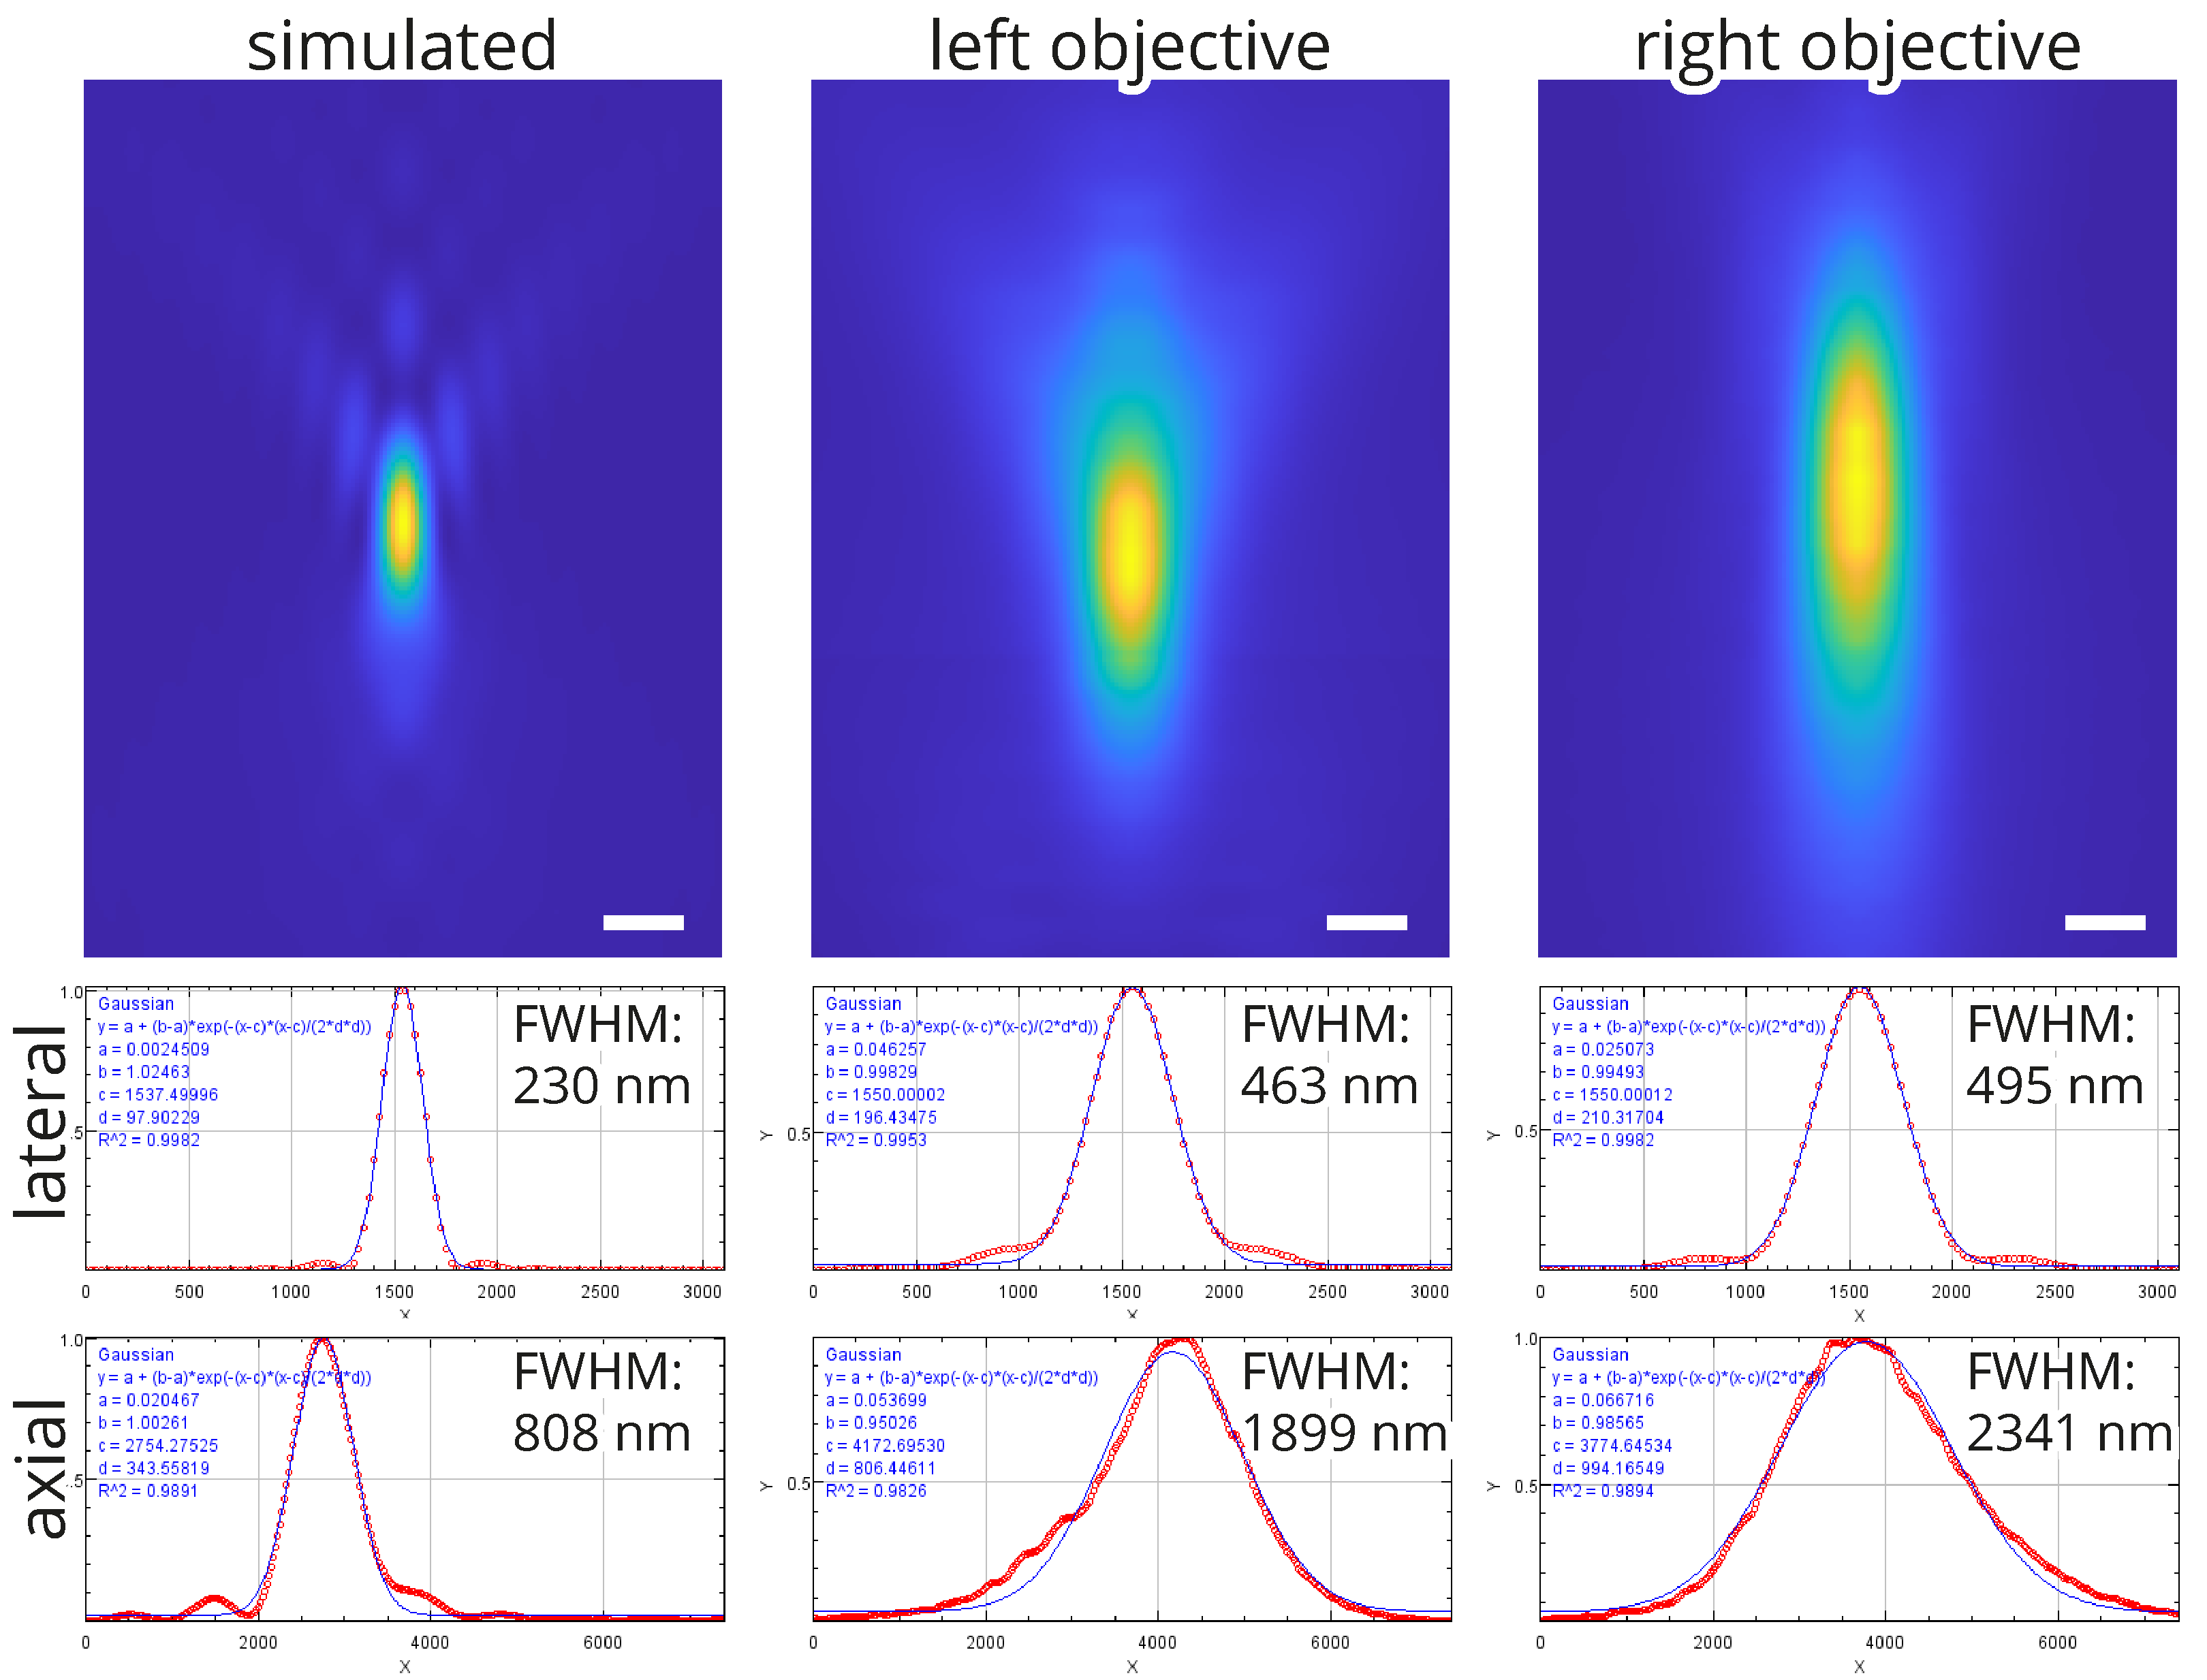
\includegraphics[width=\textwidth]{PSF}
      \bcaption[Simulated and measured PSF of Dual Mouse-SPIM]{Top row: axial sections of simulated and measured point spread functions. Middle row: lateral intensity profile and Gaussian fit. Bottom row: Axial intensity profile and Gaussian fit. Simulations were performed based on the Gibson-Lanni model. Immersion medium  and sample refractive index: 1.330, coverslip (FEP foil) refractive index: 1.344, coverslip distance: \SI{1900}{\micro m}, coverslip thickness: \SI{50}{\micro m}. Excitation wavelength: $\lambda_{ex} = \SI{561}{nm}$. Emission wavelength: $\lambda_{em} = \SI{600}{nm}$. Scale bar: \SI{1}{\micro m}.}
      \label{fig:measuredPSF}
    \end{figure}

    It is apparent from the simulations that even though the FEP refractive index is almost identical to the refractive index of water, a slight spherical aberration is still present even for the ideal case (\autoref{fig:measuredPSF}, left). The resolution measured as the FWHM of the intensity profile through the lateral and axial cross sections is \SI{271}{nm} and \SI{866}{nm} respectively. The FWHM was measured in Fiji by fitting a Gaussian curve, and multiplying the standard deviation of the resulting fit by $2 \sqrt{2 \ln 2}$.

    % \subsubsection{Methods}
    To experimentally determine the resolution of the microscope and characterize its optical performance, we measured the point spread function using fluorescently labeled beads suspended in 0.8\% GelRite (\autoref{sec:methods2}). The gel was loaded in glass capillaries  and allowed to cool. After the gel solidified, a $\sim$\SI{1}{mm} piece was cut off and placed in the microscope sample holder. The beads were imaged from both views using the \SI{561}{nm} laser line with the 561 long-pass filter (Semrock, BLP02-561R-25).

    From both views 12 beads were averaged using Fiji \cite{schindelin_fiji:_2012} and the 3D PSF estimator of the MOSAIC suite \cite{cardinale_imagej_2010}. In order to acquire a more accurate PSF, the averaged bead images were deconvolved with the ideal image of the bead (uniform sphere with a diameter of \SI{500}{nm}) using the DeconvolutionLab2 Fiji plugin \cite{sage_deconvolutionlab2:_2017}. The results of the deconvolution are shown on \autoref{fig:measuredPSF}. Similarly to the simulation, we measured the axial and lateral resolutions on the experimental PSFs. For the left view, the measured resolutions were \SI{396}{nm} in the lateral direction, and \SI{1350}{nm} in the axial direction. For the right view the lateral resolution was \SI{426}{nm}, and the axial was \SI{1297}{nm}.

    \begin{figure}
      \centering
      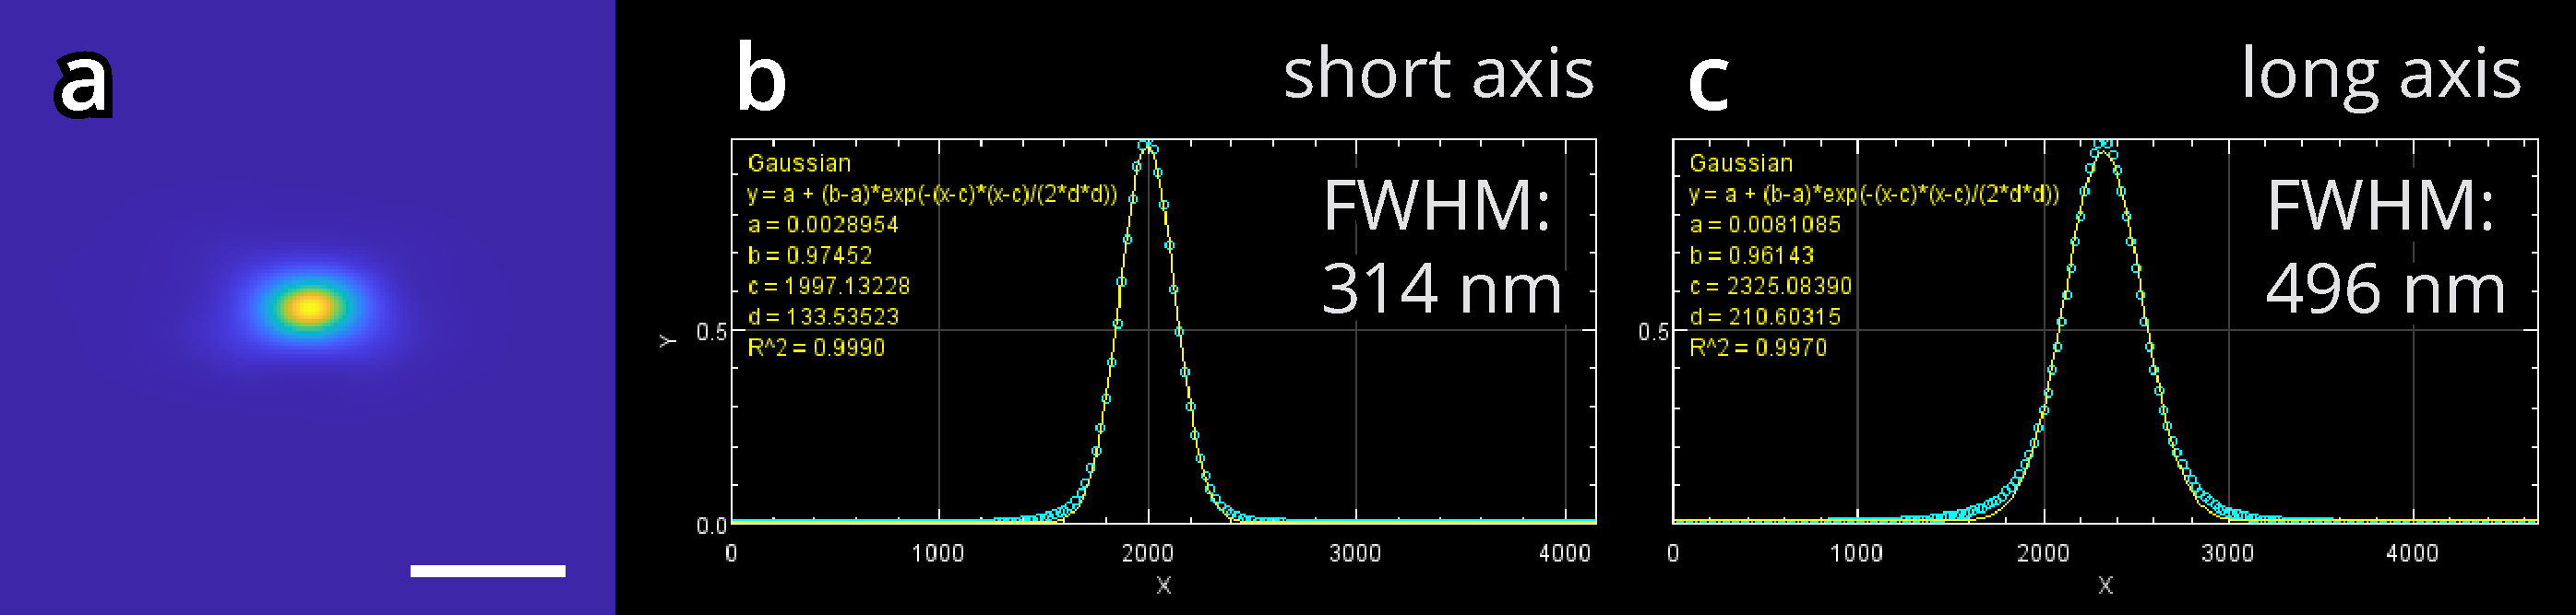
\includegraphics[width=0.9\textwidth]{beads/fusedPSF}
      \bcaption[Combined PSF of 2 views]{(\textbf{a}) The measured PSFs (\autoref{fig:measuredPSF}) were rotated to their corresponding orientations and multiplied. (\textbf{b}) Gaussian fit along the short axis of the combined PSF; FWHM=\SI{314}{nm}. (\textbf{c}) Gaussian fit along the long axis of the combined PSF; FWHM=\SI{496}{nm}. Scale bar, \SI{1}{\micro m}}
      \label{fig:fusedPSF}
    \end{figure}
    
    To estimate the achievable multi-view resolution of the system, we combined the two measured PSFs. First, the PSFs were rotated by $\pm \SI{60}{\degree}$ to correspond to the objective orientations. The PSF images were then normalized by scaling the maximum to 1, and the two rotated and normalized PSFs were multiplied (\autoref{fig:fusedPSF}). Resolution of the combined PSF is much improved in all directions: along its shortest axis the FWHM is \SI{314}{nm}, and along the longest axis the FWHM is \SI{496}{nm} (\autoref{fig:fusedPSF}). Both are better than the corresponding resolutions for a single view, especially along the long axis, where the FWHM is 2.67 times smaller. This is almost perfectly matching the theoretically expected increase in the axial direction (compare with \autoref{sec:120concept}).


  \subsubsection{Resolution inside a \textit{Drosphila melanogaster} embryo}

    Apart from measuring the point spread function and resolution in an ideal bead sample, we also wanted to know the resolution inside a biological sample, as the tissues usually introduce some aberrations to the light path. Although these aberrations highly depend on the sample, as a worst case scenario, we measured the point spread function inside a \textit{Drosophila melanogater} embryo. As this specimen is highly opaque and scattering, it gives a good estimate for the upper bound of the resolution.

    Instead of the fluorescent beads, we imaged a \textit{Drosophila} embryo expressing H2A-mCherry marking the nuclei, and ASL-YFP marking the centrioles (\autoref{fig:drosoEmbryo}a, and \autoref{sec:methods2}). As the centriolar protein ASL is diffraction limited in size \cite{gonczy_towards_2012}, its image gives a good estimate for the point spread function inside the specimen.

    Similarly to the bead recordings, 15 centriole images were averaged with the 3D PSF tool of the MOSAIC plugin in Fiji (\autoref{fig:drosoEmbryo}c). On the averaged image we measured the resolution by fitting a Gaussian function on the lateral and axial intensity profiles (\autoref{fig:drosoEmbryo}d,e), and calculating the FWHM of the fitted Gaussian. The size of the averaged centrioles was \SI{654}{nm} in the lateral, and \SI{2739}{nm} in the axial direction.

    \begin{figure}[ptb]
      \centering
      \includegraphics[width=.9\textwidth]{droso/drosoEmbryo}
      \bcaption[Maximum intensity projection of a \textit{Drosophila melanogaster} embryo recording]{Maximum intensity projection of a \SI{30}{\micro m} thick substack. Orange: nuclei (H2A-mCherry), blue: centrioles (ASL-YFP). 50x magnification. (\textbf{a}) Overview of the embryo. (\textbf{b}) Zoomed in view to the region marked in (\textbf{a}). (\textbf{c}) Average image of 15 centrioles distributed evenly in the embryo. (d) Gaussian fit on the lateral intensity profile of the averaged centrioles; FWHM=\SI{654}{nm}. (d) Gaussian fit on the axial intensity profile of the averaged centrioles; FWHM=\SI{2739}{nm}.}
      \label{fig:drosoEmbryo}
    \end{figure}
    
  \subsubsection{Multi-view imaging of a mouse zygote}
    \begin{figure}[ptb]
      \centering
      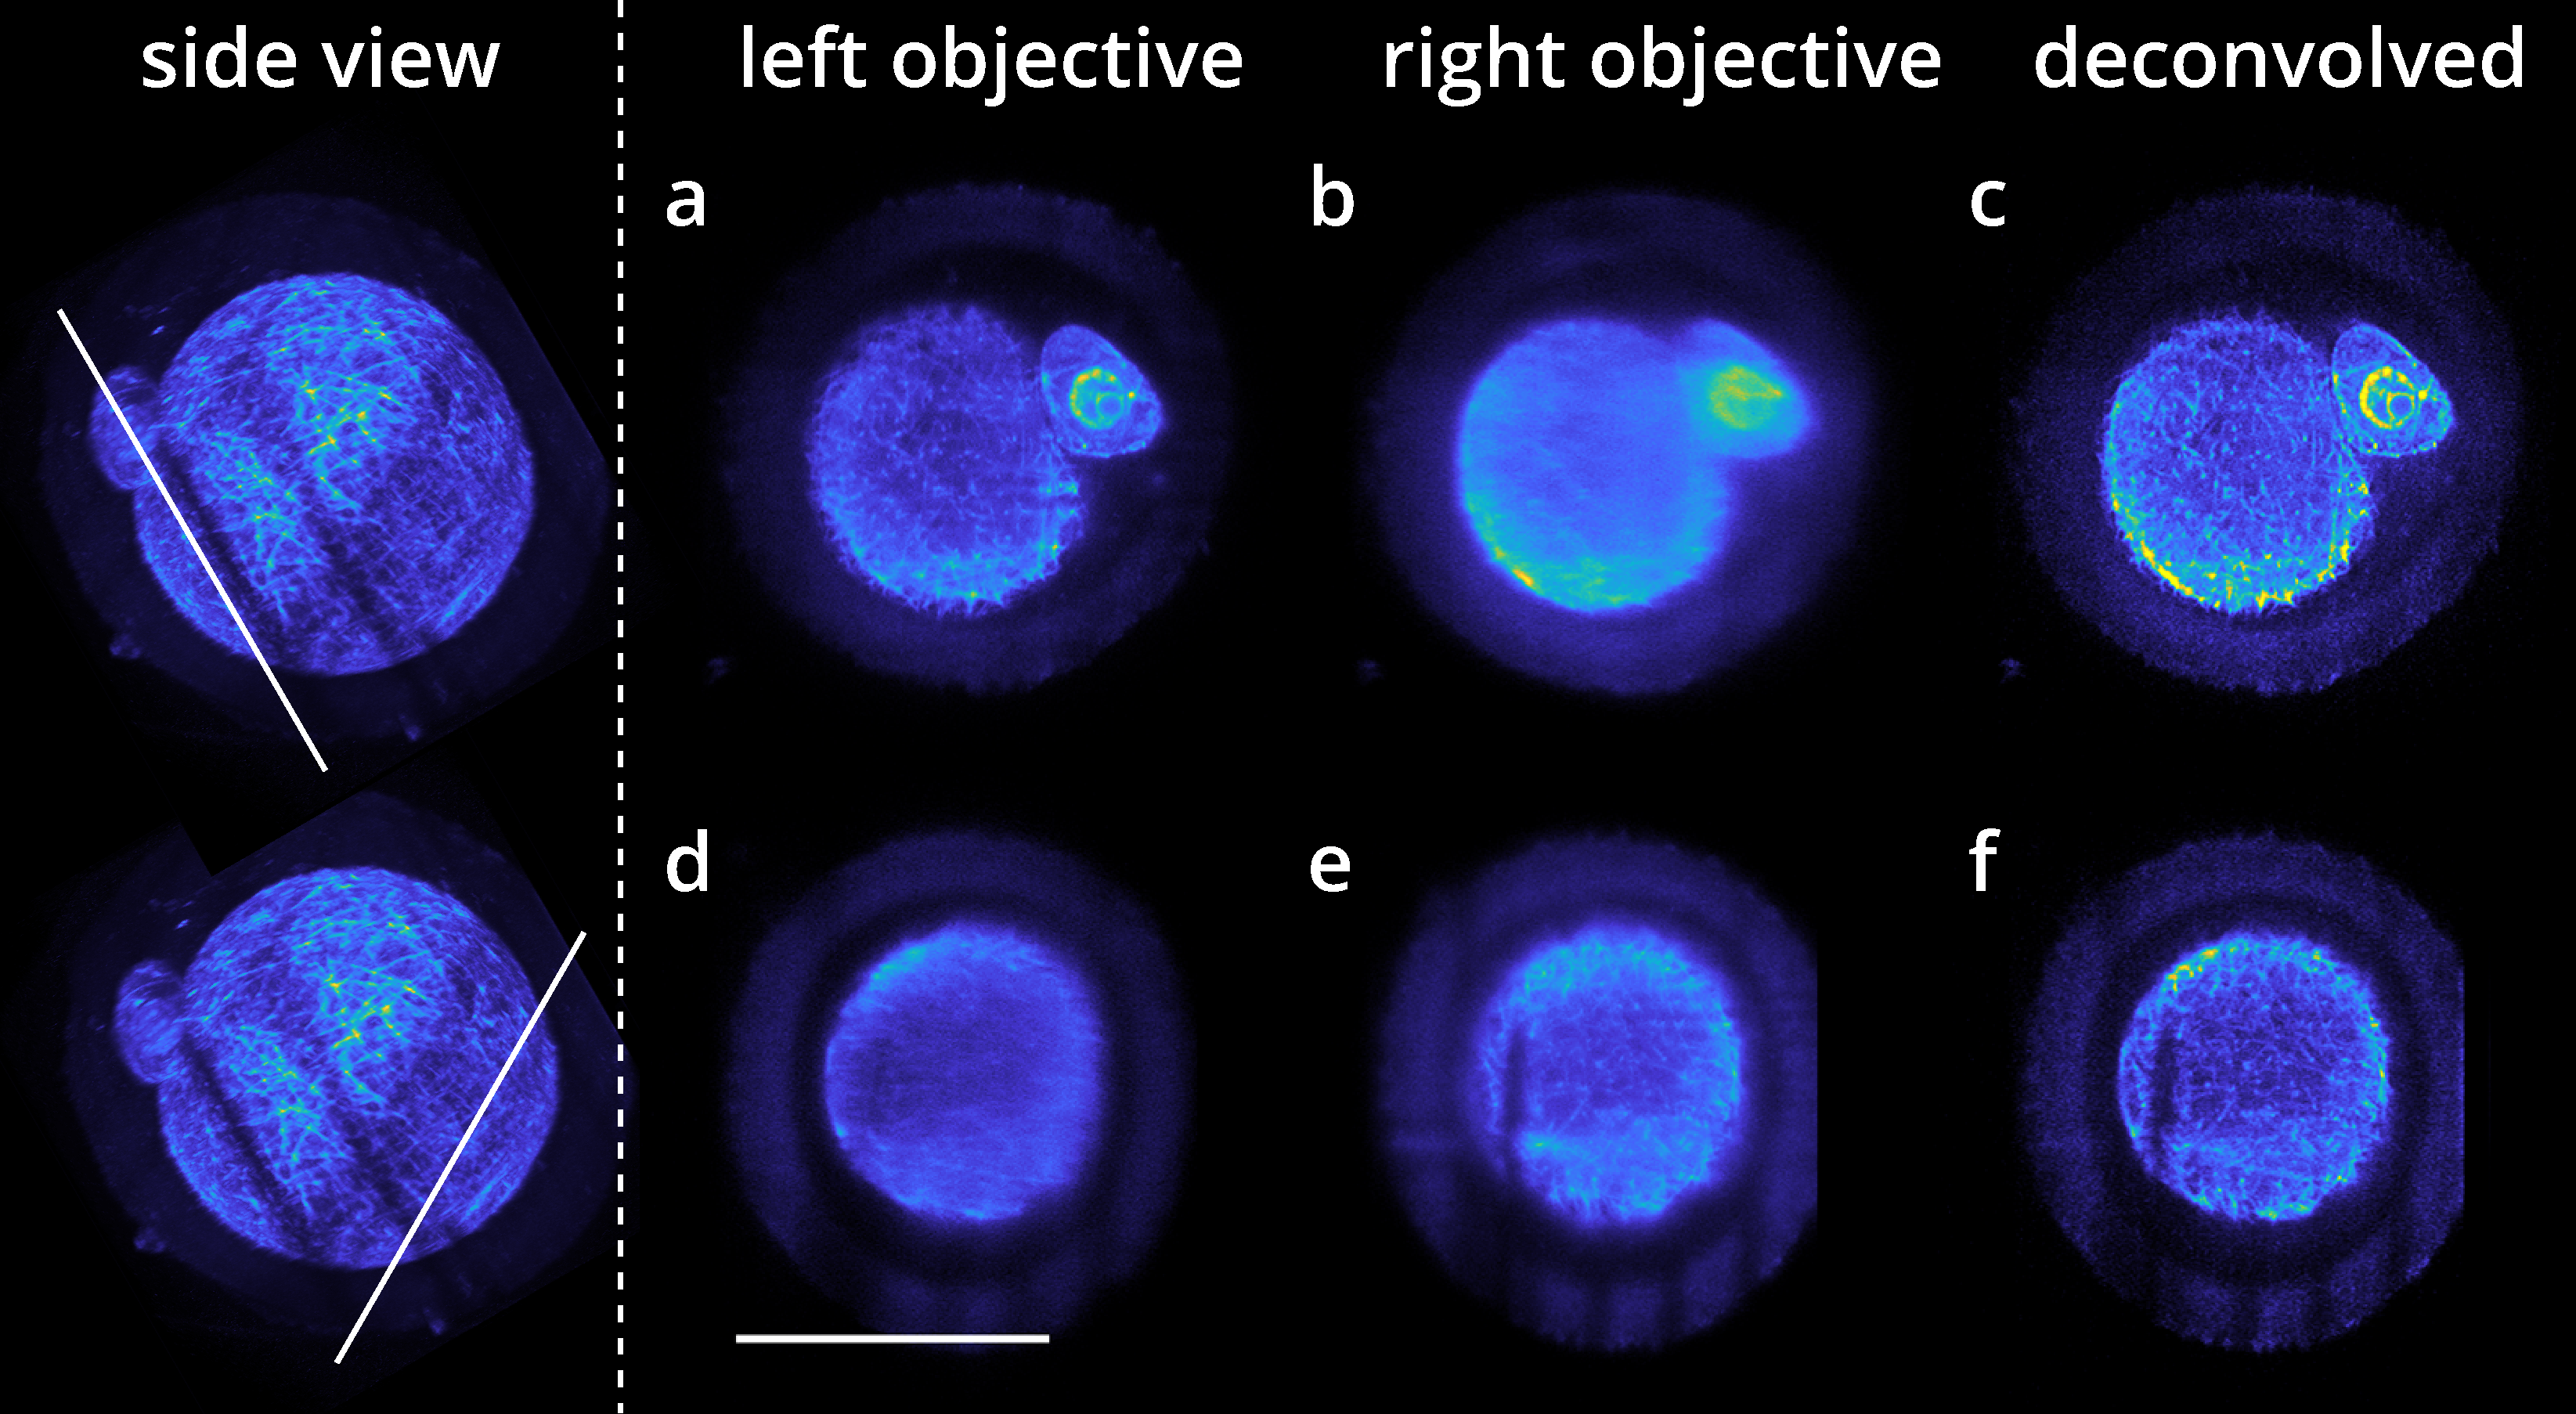
\includegraphics[width=1\textwidth]{zygoteMontage}
      \bcaption[Multi-view recording of a mouse zygote]{Dual-view imaging was performed on a fixed mouse zygote. Microtubules were stained with Alexa Fluor 488 coupled secondary antibodies. Top row: view of Left objective. Bottom row: view of Right objective. (a) Raw image from left objective. (b) Rotated view of Right objective. (c) Multi-view deconvolution of stacks (a) and (b). (d) Rotated slice from left objective. (e) Raw image from right objective. (f) Multi-view deconvolution of stacks (d) and (e). Scale bar: \SI{50}{\micro m}. The darker banding artifacts visible on the side view are due to bleaching.}
      \label{fig:zygoteMontage}
    \end{figure}

    To demonstrate the multi-view capabilities and improved image quality of the microscope, we performed dual-view imaging of a fixed mouse zygote and combined the images using the Multiview Reconstruction \cite{preibisch_efficient_2014} plugin of Fiji (\autoref{fig:zygoteMontage}). The microtubules were stained with Alexa Fluor 488 coupled secondary antibodies, and the zygote was imaged from both views with \SI{0.5}{\micro m} inter-plane distance.

    Anisotropy in the resolution becomes apparent in the single-view recordings, when the stacks are resliced from a different direction than the imaging plane. Even though the native view of each objective (\autoref{fig:zygoteMontage}a,d) shows good contrast and easy to recognize features, when rotated and sliced corresponding to the view of the other objective, the contrast is almost completely gone, and the resolution is decreased (\autoref{fig:zygoteMontage}b,e). The fused stack, after the multi-view deconvolution contains the high resolution information from both views, and thus both directions show good quality and high contrast (\autoref{fig:zygoteMontage}c,f).




  
  

  % \subsection{Drosophila salivary gland imaging}
  %   Salivary glands from third instar larvae expressing fluorescent nuclear (H2A-mCherry) and centriole (ASL-YFP) markers were kindly provided by Ulla-Maj Fiuza. The salivary glands were imaged in PBS, together with a small piece of gel with fluorescent beads.





% ########  ####  ######   ######  ##     ## 
% ##     ##  ##  ##    ## ##    ## ##     ## 
% ##     ##  ##  ##       ##       ##     ## 
% ##     ##  ##   ######  ##       ##     ## 
% ##     ##  ##        ## ##       ##     ## 
% ##     ##  ##  ##    ## ##    ## ##     ## 
% ########  ####  ######   ######   #######  

\section{Discussion}
\label{sec:discu-microscope}

  In this chapter we have presented a novel light-sheet microscope designed for subcellular imaging of mouse embryos. The microscope has two identical objectives, positioned in a \SI{120}{\degree} angle, and operates with two \SI{30}{\degree} tilted light-sheets. Due to the symmetrical design both objectives can be used for detection and illumination as well, providing multi-view capabilities without sample rotation. The \SI{120}{\degree} objective configuration allows the use of high numerical aperture objectives (1.1 instead of 0.8), which drastically increases the light collection efficiency compared to the conventional \SI{90}{\degree} configuration. Due to this improvement the microscope requires less tradeoff in imaging speed, resolution, contrast, and phototoxicity, as the corners of the pyramid (\autoref{fig:tradeoffs}) are now moved closer together.

  We have characterized the optical properties of the microscope by measuring the light-sheet dimensions (average length: \SI{93}{\micro m}, average thickness: \SI{3.6}{\micro m}), and by measuring the point spread function. When combining the two views, the resolution is much closer to an ideal isotropic shape, being \SI{496}{nm} along the long axis and \SI{314}{nm} along the short axis as opposed to \SI{1323}{nm} and \SI{411}{nm} measured for a single view. This 2.67 fold increase in axial resolution can potentially make the difference in being able to track all chromosomes in a developing mouse embryo.

  The obtained resolution is comparable to the state of the art lattice light-sheet microscopy (LLSM) \cite{chen_lattice_2014} (\SI{230}{nm} lateral and \SI{370}{nm} axial), however, the optical alignment and the operation of our microscope is considerably simpler, as there is no need for the use of a spatial light modulator. As LLSM relies on the self-interference of the illumination beam to obtain the thin sectioning pattern, the practical imaging volume is only $50 \times 50 \times \SI{50}{\micro m ^3}$. In contrast, the Dual Mouse-SPIM is capable of imaging a volume of $260 \times 100 \times \SI{100}{\micro m ^3}$ due to the more robust Gaussian-beam illumination and the two-sided detection. Imaging very fast dynamics from two directions, however, might be challenging, as the detection direction is switched with a mechanical part, which limits the maximum volumetric imaging speed.

  To be able to surpass the proof-of-concept state, the microscope still needs some improvements. The detection view switching unit needs to be improved to minimize field of view drift of both views. One possible issue with the current solution is the insufficient damping of the moving mirror unit, which can cause unwanted vibrations when the switching force is high. This can also be a possible explanation of why only one direction was unstable, as the movement speed was not equal in both directions. Since the pneumatic cylinder has a single actuator rod, the force on the piston is different depending on the movement direction: on the side where the rod is attached to the piston the surface area is smaller, thus the actuating force is lower with the same air pressure. This could be remedied by applying a more efficient damping system, and by making sure that the forces are the same in both directions. For small specimens, if a reduced field of view is sufficient, the entire moving assembly can be replaced by a fixed prism mirror, which reflects the two objective images on either half of the camera sensor. This has the added benefit of faster imaging, since the switching time between the two imaging branches is only limited by the galvanometric scanner. Another solution could be the addition of a second camera, which would make the view switching completely unnecessary without sacrificing the field of view.
  
  Another necessity for long-term experiments is the implementation of an environmental chamber to provide the appropriate conditions for live mammalian embryo imaging. This involves the integration of a heating element and a gas mixer unit to the mechanical design, complemented by an enclosure that seals off the environment of the imaging chamber. The mechanical design is already underway and the electronic control will be integrated with the modular control software.

  The use of high-NA objectives also keeps the door open for future upgrades, such as the addition of structured illumination \cite{keller_fast_2010, chang_csilsfm_2017}, or coupling in a high-power pulsed laser for photomanipulation capabilities \cite{rauzi_probing_2017}. Another natural extension to the system would be the addition of a third objective that would allow for truly isotropic imaging and two-sided sample illumination. Using three objectives would introduce some challenges in sample mounting, as the open-top sample holder design could not be used in the same way. A more practical way would be the use of an FEP tube, where the embryos could develop in the appropriate medium while they are sealed from the outside by gel plugs on either side. Of course such a system will need to be thoroughly tested of live imaging compatibility.


  Single-view solutions for isotropic imaging only allow a very limited field of view. For diffraction-limited optical sectioning a Gaussian beam is diverging too fast \cite{dean_diagonally_2016}, while the use of other, non-diffractive beams rely on self-interference \cite{chen_lattice_2014}, which breaks down after a few tens of micrometers inside the sample. Our dual-view high NA solution allows for near isotropic resolution even for large fields of view, such as for entire mouse zygotes or embryos (\SI{120}{\micro m}\texttimes\SI{120}{\micro m}\texttimes\SI{120}{\micro m}).
  